% Seminarul 4: Probabilitate
% Statistica piețelor financiare -- Program de licență, Academia de Studii Economice din București
% GENERAT de latex/build_seminar4.py -- modificați generatorul, nu acest fișier.
% Implicit versiunea pentru studenți; versiunea profesorului este wrapper-ul *_solutions.tex.
\makeatletter\@ifundefined{ifsolutions}{\expandafter\newif\csname ifsolutions\endcsname}{}\makeatother

\newcommand{\coursename}{Statistica piețelor financiare}
\def\sfmlang{ro}
% Preambul comun SFM -- Statistica piețelor financiare / Statistics of Financial Markets (Beamer, 16:9)
% Același design ca MFM. Înainte de % Preambul comun SFM -- Statistica piețelor financiare / Statistics of Financial Markets (Beamer, 16:9)
% Același design ca MFM. Înainte de % Preambul comun SFM -- Statistica piețelor financiare / Statistics of Financial Markets (Beamer, 16:9)
% Același design ca MFM. Înainte de \input{../../latex/preamble} se definește
%   \newcommand{\coursename}{Statistics of Financial Markets}      (EN)
%   \newcommand{\coursename}{Statistica piețelor financiare}       (RO)  și  \def\sfmlang{ro}
% Fișierele .tex se află în EN/Courses, EN/Seminars, RO/Cursuri, RO/Seminarii (două niveluri sub rădăcină).
% Deck-urile sînt generate de latex/build_chapterN.py / build_seminarN.py (vezi latex/sfm_build.py).

\documentclass[9pt, aspectratio=169, t]{beamer}
\providecommand{\coursename}{Statistics of Financial Markets}

% Ensure content fits on slides
\setbeamersize{text margin left=8mm, text margin right=8mm}

%=============================================================================
% THEME AND STYLE CONFIGURATION
%=============================================================================
\usetheme{default}
% Using default theme for clean header/footer control

% Color Palette (matching Redispatch PDF)
\definecolor{MainBlue}{RGB}{26, 58, 110}
\definecolor{AccentBlue}{RGB}{26, 58, 110}
\definecolor{IDAred}{RGB}{205, 0, 0}
\definecolor{DarkGray}{RGB}{51, 51, 51}
\definecolor{MediumGray}{RGB}{128, 128, 128}
\definecolor{LightGray}{RGB}{248, 248, 248}
\definecolor{VeryLightGray}{RGB}{235, 235, 235}
\definecolor{KeynoteGray}{RGB}{218, 218, 218}
\definecolor{SectionGray}{RGB}{120, 120, 120}
\definecolor{FooterGray}{RGB}{100, 100, 100}
\definecolor{Crimson}{RGB}{220, 53, 69}
\definecolor{Forest}{RGB}{46, 125, 50}
\definecolor{Amber}{RGB}{181, 133, 63}
\definecolor{Orange}{RGB}{230, 126, 34}
\definecolor{Purple}{RGB}{142, 68, 173}

% Gradient background (exact Keynote 315° gradient: white to RGB 218,218,218)
\setbeamertemplate{background}{%
    \begin{tikzpicture}[remember picture, overlay]
        \shade[shading=axis, shading angle=315,
        top color=white, bottom color=KeynoteGray]
        (current page.south west) rectangle (current page.north east);
    \end{tikzpicture}%
}
% Fallback solid color for compatibility
\setbeamercolor{background canvas}{bg=}

\setbeamercolor{palette primary}{bg=MainBlue, fg=white}
\setbeamercolor{palette secondary}{bg=MainBlue!85, fg=white}
\setbeamercolor{palette tertiary}{bg=MainBlue!70, fg=white}
\setbeamercolor{structure}{fg=MainBlue}
\setbeamercolor{title}{fg=IDAred}
\setbeamercolor{frametitle}{fg=IDAred, bg=}
\setbeamercolor{block title}{bg=MainBlue, fg=white}
\setbeamercolor{block body}{bg=VeryLightGray, fg=DarkGray}
\setbeamercolor{block title alerted}{bg=Crimson, fg=white}
\setbeamercolor{block body alerted}{bg=Crimson!8, fg=DarkGray}
\setbeamercolor{block title example}{bg=Forest, fg=white}
\setbeamercolor{block body example}{bg=Forest!8, fg=DarkGray}
\setbeamercolor{item}{fg=MainBlue}

% Footer colors (override Madrid theme blue)
\setbeamercolor{author in head/foot}{fg=FooterGray, bg=}
\setbeamercolor{title in head/foot}{fg=FooterGray, bg=}
\setbeamercolor{date in head/foot}{fg=FooterGray, bg=}
\setbeamercolor{section in head/foot}{fg=FooterGray, bg=}
\setbeamercolor{subsection in head/foot}{fg=FooterGray, bg=}

% Bullet styles (apply everywhere including blocks)
\setbeamertemplate{itemize item}{\color{MainBlue}$\boxdot$}
\setbeamertemplate{itemize subitem}{\color{MainBlue}$\blacktriangleright$}
\setbeamertemplate{itemize subsubitem}{\color{MainBlue}\tiny$\bullet$}
\setbeamertemplate{itemize/enumerate body begin}{\normalsize}
\setbeamertemplate{itemize/enumerate subbody begin}{\normalsize}

% Item spacing - compact style
\setlength{\leftmargini}{10pt}       % Level 1: minimal indent
\setlength{\leftmarginii}{10pt}      % Level 2: minimal additional indent
% Compact list spacing (zero extra space before/after lists in blocks)
\makeatletter
\def\@listi{\leftmargin\leftmargini \topsep 0pt \parsep 0pt \itemsep 0pt}
\def\@listii{\leftmargin\leftmarginii \topsep 0pt \parsep 0pt \itemsep 0pt}
\makeatother

\setbeamertemplate{navigation symbols}{}

%=============================================================================
% CUSTOM HEADLINE
%=============================================================================
\setbeamertemplate{headline}{%
    \vskip10pt%
    \hbox to \paperwidth{%
        \hskip0.5cm%
        {\small\color{FooterGray}\renewcommand{\hyperlink}[2]{##2}\insertsectionhead}%
        \hfill%
        \textcolor{FooterGray}{\small\insertframenumber}%
        \hskip0.5cm%
    }%
    \vskip4pt%
    {\color{FooterGray}\hrule height 0.4pt}%
}

%=============================================================================
% CUSTOM FOOTER
%=============================================================================
\usepackage{fontawesome5}

\setbeamertemplate{footline}{%
    {\color{FooterGray}\hrule height 0.4pt}%
    \vskip4pt%
    \hbox to \paperwidth{%
        \hskip0.5cm%
        \textcolor{FooterGray}{\small\coursename}%
        \hfill%
        \raisebox{-0.1em}{%
            \begin{tikzpicture}[x=0.08em, y=0.08em, line width=0.4pt]
                \draw[FooterGray] (0,3) -- (1,4) -- (2,3.5) -- (3,5) -- (4,4) -- (5,6) -- (6,5.5) -- (7,4) -- (8,5) -- (9,7) -- (10,6) -- (11,5) -- (12,6.5) -- (13,8) -- (14,7) -- (15,6) -- (16,7.5) -- (17,9) -- (18,8) -- (19,7) -- (20,8.5) -- (21,10) -- (22,9) -- (23,8) -- (24,9.5);
            \end{tikzpicture}%
        }%
        \hskip0.5cm%
    }%
    \vskip6pt%
}

%=============================================================================
% PACKAGES
%=============================================================================
\usepackage[utf8]{inputenc}
\DeclareUnicodeCharacter{03B1}{\ensuremath{\alpha}}
\usepackage[T1]{fontenc}
\usepackage{amsmath, amssymb, amsthm}
\usepackage{mathtools}
\usepackage{bm}
\usepackage{tikz}
\usetikzlibrary{arrows.meta, positioning, shapes, calc, decorations.pathreplacing, shadings}
\usepackage{booktabs}
\usepackage{multirow}
\usepackage{array}
\usepackage{graphicx}
\usepackage{hyperref}
\usepackage{colortbl}
\usepackage{listings}
\lstset{language=Python, basicstyle=\ttfamily\scriptsize, keywordstyle=\color{MainBlue}\bfseries,
  commentstyle=\color{Forest}, stringstyle=\color{Crimson}, breaklines=true,
  frame=none, backgroundcolor=\color{VeryLightGray}, xleftmargin=2mm}
\hypersetup{colorlinks=true, linkcolor=MainBlue, urlcolor=MainBlue}
\graphicspath{{../../logos/}{../../charts/}{../../photos/}}
\usepackage{xcolor}
\hfuzz=2pt  % Suppress tiny overfull warnings (<2pt)
\vfuzz=2pt  % Suppress tiny vertical overfull warnings (<2pt)

%=============================================================================
% QUANTLET COMMANDS
%   \quantlet{<displayed name>}{<url>}       (generic, compatible with the older SFM decks)
%   \sfmquantlet{Ch_05}{SFM_ch5_garch}       -> https://github.com/danpele/SFM/tree/main/Quantlets/Ch_05/SFM_ch5_garch
%   \qlurl{<folder>} is defined per chapter by the generator (Quantlets/Ch_NN/<folder>)
%=============================================================================
\newcommand{\sfmrepo}{https://github.com/danpele/SFM}
\newcommand{\sfmqlbase}{https://github.com/danpele/SFM/tree/main/Quantlets}
\newcommand{\quantlet}[2]{%
    \hfill\href{#2}{%
        \raisebox{-0.15em}{
\includegraphics[height=0.7em]{ql_logo.png}}%
        \textcolor{MainBlue}{\tiny\ #1}%
    }%
}
\newcommand{\sfmquantlet}[2]{\quantlet{\detokenize{#2}}{\sfmqlbase/#1/#2}}

%=============================================================================
% NOTEBOOKS (Google Colab)
%   \colaburl{notebooks/EN/chapter5_seminar_notebook.ipynb} -> the Colab link of a file in the SFM repo
%   \nb: the chapter notebook (each seminar deck redefines it with \renewcommand)
%=============================================================================
\newcommand{\colaburl}[1]{https://colab.research.google.com/github/danpele/SFM/blob/main/#1}
\newcommand{\nb}{https://colab.research.google.com/github/danpele/SFM/tree/main/notebooks/EN}
\newcommand{\nbname}{notebooks/EN}

%=============================================================================
% SLIDE HELPERS (used by the generators; the same as in MFM)
%=============================================================================
% local font size for list bodies (the preamble forces \normalsize)
\newcommand{\itemsize}[1]{\setbeamertemplate{itemize/enumerate body begin}{#1}\setbeamertemplate{itemize/enumerate subbody begin}{#1}}
\newcommand{\intitle}[1]{{\hypersetup{urlcolor=white}#1}}   % white links inside coloured title bars
\newcommand{\imgcap}[1]{{\scriptsize #1}\\[0.5mm]}          % caption under a photo
\newcommand{\imgcredit}[2]{{\tiny\color{FooterGray}\href{#1}{#2}}}   % image credit: source URL, author/licence
\newcommand{\aiprompt}[1]{{\ttfamily\color{MainBlue}#1}}     % a prompt to an AI assistant

%=============================================================================
% SEMINARS: student version by default; the instructor wrapper *_solutions.tex sets \solutionstrue
%=============================================================================
\makeatletter\@ifundefined{ifsolutions}{\expandafter\newif\csname ifsolutions\endcsname}{}\makeatother
\newcommand{\solonly}[1]{\ifsolutions #1\fi}
\newcommand{\propsub}{\ifsolutions\else\framesubtitle{\ifdefined\sfmlang Rezolvarea se discută la seminar\else Solution discussed in class\fi}\fi}

%=============================================================================
% APPENDIX AND CHAPTER LINKS (latex/appendix_links.py writes the calls; it also re-declares these
% macros before \begin{document}, so the decks compile with or without this preamble block)
%=============================================================================
\providecommand{\sfmapplink}[3]{\hypertarget{#2}{}\hyperlink{#1}{\beamergotobutton{#3}}}
\providecommand{\sfmappback}[2]{\begin{tikzpicture}[remember picture,overlay]\node[anchor=south east] at ([xshift=-3mm,yshift=7mm]current page.south east){\hyperlink{#1}{\beamerreturnbutton{#2}}};\end{tikzpicture}}
\providecommand{\sfmchlink}[2]{\href{#1}{#2}}
\providecommand{\sfmchlinkt}[2]{\href{#1}{\usebeamercolor[fg]{frametitle}#2}}

%=============================================================================
% QUANTINAR COMMAND: link către un curs Quantinar (subiecte avansate)
%=============================================================================
\newcommand{\quantinar}[2]{%
    \href{#2}{%
        \raisebox{-0.15em}{
\includegraphics[height=0.8em]{qr_logo.png}}%
        \textcolor{MainBlue}{\scriptsize\ #1}%
    }%
}

%=============================================================================
% CUSTOM TITLE PAGE
%=============================================================================
\defbeamertemplate*{title page}{hybrid}[1][]
{
    \vspace{0.2cm}
    % Logos row - top header (with clickable links)
    \begin{center}
        \href{https://www.ase.ro}{
\includegraphics[height=1.0cm]{ase_logo.png}}\hspace{0.3cm}%
        \href{https://theida.net}{
\includegraphics[height=1.0cm]{ida_logo.png}}\hspace{0.3cm}%
        \href{https://blockchain-research-center.com}{
\includegraphics[height=1.0cm]{brc_logo.png}}\hspace{0.3cm}%
        \href{https://www.ai4efin.ase.ro}{
\includegraphics[height=1.0cm]{ai4efin_logo.png}}\hspace{0.3cm}%
        \href{https://ipe.ro/new}{
\includegraphics[height=1.0cm]{acad_logo.png}}\hspace{0.3cm}%
        \href{https://www.digital-finance-msca.com}{
\includegraphics[height=1.0cm]{msca_logo.png}}%
    \end{center}

    \vspace{0.6cm}

    % Main title with Q logos on sides (with clickable links)
    \begin{center}
        \begin{minipage}{0.1\textwidth}
            \centering
            \href{https://quantlet.com}{
\includegraphics[height=1.1cm]{ql_logo.png}}
        \end{minipage}%
        \begin{minipage}{0.78\textwidth}
            \centering
            {\LARGE\bfseries\usebeamercolor[fg]{title}\inserttitle}

            \vspace{0.3cm}

            {\usebeamerfont{subtitle}\usebeamercolor[fg]{title}\insertsubtitle}
        \end{minipage}%
        \begin{minipage}{0.1\textwidth}
            \centering
            \href{https://quantinar.com}{
\includegraphics[height=1.1cm]{qr_logo.png}}
        \end{minipage}
    \end{center}

    \vspace{0.6cm}

    % Authors (left aligned)
    \hspace{0.5cm}{\usebeamerfont{author}\insertauthor}

    \vspace{0.3cm}

    % Institute/Affiliations (left aligned)
    \hspace{0.5cm}\begin{minipage}[t]{0.9\textwidth}
        \raggedright\small\insertinstitute
    \end{minipage}
}

%=============================================================================
% THEOREM ENVIRONMENTS
%=============================================================================
\theoremstyle{definition}
\setbeamertemplate{theorems}[numbered]
\ifdefined\sfmlang
\newtheorem{defn}{Definiție}
\newtheorem{thm}{Teoremă}
\newtheorem{prop}{Propoziție}
\newtheorem{rmk}{Observație}
\else
\newtheorem{defn}{Definition}
\newtheorem{thm}{Theorem}
\newtheorem{prop}{Proposition}
\newtheorem{rmk}{Remark}
\fi

%=============================================================================
% CENTRED MINIPAGE (no extra vertical space)
%=============================================================================
\newenvironment{cminipage}[1]{%
    \par\noindent\hfill\begin{minipage}{#1}\ignorespaces
}{%
    \end{minipage}\hfill\null\par
}

%=============================================================================
% CUSTOM COMMANDS
%=============================================================================
\newcommand{\E}{\mathbb{E}}
\newcommand{\Var}{\text{Var}}
\newcommand{\Cov}{\text{Cov}}
\newcommand{\Corr}{\text{Corr}}
\newcommand{\R}{\mathbb{R}}
\newcommand{\N}{\mathbb{N}}
\newcommand{\Z}{\mathbb{Z}}
\newcommand{\B}{\mathbf{B}}
\newcommand{\imark}{\textcolor{MainBlue}{\textbullet}}
\newcommand{\RMSE}{\text{RMSE}}
\newcommand{\MAE}{\text{MAE}}
\newcommand{\MAPE}{\text{MAPE}}

 se definește
%   \newcommand{\coursename}{Statistics of Financial Markets}      (EN)
%   \newcommand{\coursename}{Statistica piețelor financiare}       (RO)  și  \def\sfmlang{ro}
% Fișierele .tex se află în EN/Courses, EN/Seminars, RO/Cursuri, RO/Seminarii (două niveluri sub rădăcină).
% Deck-urile sînt generate de latex/build_chapterN.py / build_seminarN.py (vezi latex/sfm_build.py).

\documentclass[9pt, aspectratio=169, t]{beamer}
\providecommand{\coursename}{Statistics of Financial Markets}

% Ensure content fits on slides
\setbeamersize{text margin left=8mm, text margin right=8mm}

%=============================================================================
% THEME AND STYLE CONFIGURATION
%=============================================================================
\usetheme{default}
% Using default theme for clean header/footer control

% Color Palette (matching Redispatch PDF)
\definecolor{MainBlue}{RGB}{26, 58, 110}
\definecolor{AccentBlue}{RGB}{26, 58, 110}
\definecolor{IDAred}{RGB}{205, 0, 0}
\definecolor{DarkGray}{RGB}{51, 51, 51}
\definecolor{MediumGray}{RGB}{128, 128, 128}
\definecolor{LightGray}{RGB}{248, 248, 248}
\definecolor{VeryLightGray}{RGB}{235, 235, 235}
\definecolor{KeynoteGray}{RGB}{218, 218, 218}
\definecolor{SectionGray}{RGB}{120, 120, 120}
\definecolor{FooterGray}{RGB}{100, 100, 100}
\definecolor{Crimson}{RGB}{220, 53, 69}
\definecolor{Forest}{RGB}{46, 125, 50}
\definecolor{Amber}{RGB}{181, 133, 63}
\definecolor{Orange}{RGB}{230, 126, 34}
\definecolor{Purple}{RGB}{142, 68, 173}

% Gradient background (exact Keynote 315° gradient: white to RGB 218,218,218)
\setbeamertemplate{background}{%
    \begin{tikzpicture}[remember picture, overlay]
        \shade[shading=axis, shading angle=315,
        top color=white, bottom color=KeynoteGray]
        (current page.south west) rectangle (current page.north east);
    \end{tikzpicture}%
}
% Fallback solid color for compatibility
\setbeamercolor{background canvas}{bg=}

\setbeamercolor{palette primary}{bg=MainBlue, fg=white}
\setbeamercolor{palette secondary}{bg=MainBlue!85, fg=white}
\setbeamercolor{palette tertiary}{bg=MainBlue!70, fg=white}
\setbeamercolor{structure}{fg=MainBlue}
\setbeamercolor{title}{fg=IDAred}
\setbeamercolor{frametitle}{fg=IDAred, bg=}
\setbeamercolor{block title}{bg=MainBlue, fg=white}
\setbeamercolor{block body}{bg=VeryLightGray, fg=DarkGray}
\setbeamercolor{block title alerted}{bg=Crimson, fg=white}
\setbeamercolor{block body alerted}{bg=Crimson!8, fg=DarkGray}
\setbeamercolor{block title example}{bg=Forest, fg=white}
\setbeamercolor{block body example}{bg=Forest!8, fg=DarkGray}
\setbeamercolor{item}{fg=MainBlue}

% Footer colors (override Madrid theme blue)
\setbeamercolor{author in head/foot}{fg=FooterGray, bg=}
\setbeamercolor{title in head/foot}{fg=FooterGray, bg=}
\setbeamercolor{date in head/foot}{fg=FooterGray, bg=}
\setbeamercolor{section in head/foot}{fg=FooterGray, bg=}
\setbeamercolor{subsection in head/foot}{fg=FooterGray, bg=}

% Bullet styles (apply everywhere including blocks)
\setbeamertemplate{itemize item}{\color{MainBlue}$\boxdot$}
\setbeamertemplate{itemize subitem}{\color{MainBlue}$\blacktriangleright$}
\setbeamertemplate{itemize subsubitem}{\color{MainBlue}\tiny$\bullet$}
\setbeamertemplate{itemize/enumerate body begin}{\normalsize}
\setbeamertemplate{itemize/enumerate subbody begin}{\normalsize}

% Item spacing - compact style
\setlength{\leftmargini}{10pt}       % Level 1: minimal indent
\setlength{\leftmarginii}{10pt}      % Level 2: minimal additional indent
% Compact list spacing (zero extra space before/after lists in blocks)
\makeatletter
\def\@listi{\leftmargin\leftmargini \topsep 0pt \parsep 0pt \itemsep 0pt}
\def\@listii{\leftmargin\leftmarginii \topsep 0pt \parsep 0pt \itemsep 0pt}
\makeatother

\setbeamertemplate{navigation symbols}{}

%=============================================================================
% CUSTOM HEADLINE
%=============================================================================
\setbeamertemplate{headline}{%
    \vskip10pt%
    \hbox to \paperwidth{%
        \hskip0.5cm%
        {\small\color{FooterGray}\renewcommand{\hyperlink}[2]{##2}\insertsectionhead}%
        \hfill%
        \textcolor{FooterGray}{\small\insertframenumber}%
        \hskip0.5cm%
    }%
    \vskip4pt%
    {\color{FooterGray}\hrule height 0.4pt}%
}

%=============================================================================
% CUSTOM FOOTER
%=============================================================================
\usepackage{fontawesome5}

\setbeamertemplate{footline}{%
    {\color{FooterGray}\hrule height 0.4pt}%
    \vskip4pt%
    \hbox to \paperwidth{%
        \hskip0.5cm%
        \textcolor{FooterGray}{\small\coursename}%
        \hfill%
        \raisebox{-0.1em}{%
            \begin{tikzpicture}[x=0.08em, y=0.08em, line width=0.4pt]
                \draw[FooterGray] (0,3) -- (1,4) -- (2,3.5) -- (3,5) -- (4,4) -- (5,6) -- (6,5.5) -- (7,4) -- (8,5) -- (9,7) -- (10,6) -- (11,5) -- (12,6.5) -- (13,8) -- (14,7) -- (15,6) -- (16,7.5) -- (17,9) -- (18,8) -- (19,7) -- (20,8.5) -- (21,10) -- (22,9) -- (23,8) -- (24,9.5);
            \end{tikzpicture}%
        }%
        \hskip0.5cm%
    }%
    \vskip6pt%
}

%=============================================================================
% PACKAGES
%=============================================================================
\usepackage[utf8]{inputenc}
\DeclareUnicodeCharacter{03B1}{\ensuremath{\alpha}}
\usepackage[T1]{fontenc}
\usepackage{amsmath, amssymb, amsthm}
\usepackage{mathtools}
\usepackage{bm}
\usepackage{tikz}
\usetikzlibrary{arrows.meta, positioning, shapes, calc, decorations.pathreplacing, shadings}
\usepackage{booktabs}
\usepackage{multirow}
\usepackage{array}
\usepackage{graphicx}
\usepackage{hyperref}
\usepackage{colortbl}
\usepackage{listings}
\lstset{language=Python, basicstyle=\ttfamily\scriptsize, keywordstyle=\color{MainBlue}\bfseries,
  commentstyle=\color{Forest}, stringstyle=\color{Crimson}, breaklines=true,
  frame=none, backgroundcolor=\color{VeryLightGray}, xleftmargin=2mm}
\hypersetup{colorlinks=true, linkcolor=MainBlue, urlcolor=MainBlue}
\graphicspath{{../../logos/}{../../charts/}{../../photos/}}
\usepackage{xcolor}
\hfuzz=2pt  % Suppress tiny overfull warnings (<2pt)
\vfuzz=2pt  % Suppress tiny vertical overfull warnings (<2pt)

%=============================================================================
% QUANTLET COMMANDS
%   \quantlet{<displayed name>}{<url>}       (generic, compatible with the older SFM decks)
%   \sfmquantlet{Ch_05}{SFM_ch5_garch}       -> https://github.com/danpele/SFM/tree/main/Quantlets/Ch_05/SFM_ch5_garch
%   \qlurl{<folder>} is defined per chapter by the generator (Quantlets/Ch_NN/<folder>)
%=============================================================================
\newcommand{\sfmrepo}{https://github.com/danpele/SFM}
\newcommand{\sfmqlbase}{https://github.com/danpele/SFM/tree/main/Quantlets}
\newcommand{\quantlet}[2]{%
    \hfill\href{#2}{%
        \raisebox{-0.15em}{
\includegraphics[height=0.7em]{ql_logo.png}}%
        \textcolor{MainBlue}{\tiny\ #1}%
    }%
}
\newcommand{\sfmquantlet}[2]{\quantlet{\detokenize{#2}}{\sfmqlbase/#1/#2}}

%=============================================================================
% NOTEBOOKS (Google Colab)
%   \colaburl{notebooks/EN/chapter5_seminar_notebook.ipynb} -> the Colab link of a file in the SFM repo
%   \nb: the chapter notebook (each seminar deck redefines it with \renewcommand)
%=============================================================================
\newcommand{\colaburl}[1]{https://colab.research.google.com/github/danpele/SFM/blob/main/#1}
\newcommand{\nb}{https://colab.research.google.com/github/danpele/SFM/tree/main/notebooks/EN}
\newcommand{\nbname}{notebooks/EN}

%=============================================================================
% SLIDE HELPERS (used by the generators; the same as in MFM)
%=============================================================================
% local font size for list bodies (the preamble forces \normalsize)
\newcommand{\itemsize}[1]{\setbeamertemplate{itemize/enumerate body begin}{#1}\setbeamertemplate{itemize/enumerate subbody begin}{#1}}
\newcommand{\intitle}[1]{{\hypersetup{urlcolor=white}#1}}   % white links inside coloured title bars
\newcommand{\imgcap}[1]{{\scriptsize #1}\\[0.5mm]}          % caption under a photo
\newcommand{\imgcredit}[2]{{\tiny\color{FooterGray}\href{#1}{#2}}}   % image credit: source URL, author/licence
\newcommand{\aiprompt}[1]{{\ttfamily\color{MainBlue}#1}}     % a prompt to an AI assistant

%=============================================================================
% SEMINARS: student version by default; the instructor wrapper *_solutions.tex sets \solutionstrue
%=============================================================================
\makeatletter\@ifundefined{ifsolutions}{\expandafter\newif\csname ifsolutions\endcsname}{}\makeatother
\newcommand{\solonly}[1]{\ifsolutions #1\fi}
\newcommand{\propsub}{\ifsolutions\else\framesubtitle{\ifdefined\sfmlang Rezolvarea se discută la seminar\else Solution discussed in class\fi}\fi}

%=============================================================================
% APPENDIX AND CHAPTER LINKS (latex/appendix_links.py writes the calls; it also re-declares these
% macros before \begin{document}, so the decks compile with or without this preamble block)
%=============================================================================
\providecommand{\sfmapplink}[3]{\hypertarget{#2}{}\hyperlink{#1}{\beamergotobutton{#3}}}
\providecommand{\sfmappback}[2]{\begin{tikzpicture}[remember picture,overlay]\node[anchor=south east] at ([xshift=-3mm,yshift=7mm]current page.south east){\hyperlink{#1}{\beamerreturnbutton{#2}}};\end{tikzpicture}}
\providecommand{\sfmchlink}[2]{\href{#1}{#2}}
\providecommand{\sfmchlinkt}[2]{\href{#1}{\usebeamercolor[fg]{frametitle}#2}}

%=============================================================================
% QUANTINAR COMMAND: link către un curs Quantinar (subiecte avansate)
%=============================================================================
\newcommand{\quantinar}[2]{%
    \href{#2}{%
        \raisebox{-0.15em}{
\includegraphics[height=0.8em]{qr_logo.png}}%
        \textcolor{MainBlue}{\scriptsize\ #1}%
    }%
}

%=============================================================================
% CUSTOM TITLE PAGE
%=============================================================================
\defbeamertemplate*{title page}{hybrid}[1][]
{
    \vspace{0.2cm}
    % Logos row - top header (with clickable links)
    \begin{center}
        \href{https://www.ase.ro}{
\includegraphics[height=1.0cm]{ase_logo.png}}\hspace{0.3cm}%
        \href{https://theida.net}{
\includegraphics[height=1.0cm]{ida_logo.png}}\hspace{0.3cm}%
        \href{https://blockchain-research-center.com}{
\includegraphics[height=1.0cm]{brc_logo.png}}\hspace{0.3cm}%
        \href{https://www.ai4efin.ase.ro}{
\includegraphics[height=1.0cm]{ai4efin_logo.png}}\hspace{0.3cm}%
        \href{https://ipe.ro/new}{
\includegraphics[height=1.0cm]{acad_logo.png}}\hspace{0.3cm}%
        \href{https://www.digital-finance-msca.com}{
\includegraphics[height=1.0cm]{msca_logo.png}}%
    \end{center}

    \vspace{0.6cm}

    % Main title with Q logos on sides (with clickable links)
    \begin{center}
        \begin{minipage}{0.1\textwidth}
            \centering
            \href{https://quantlet.com}{
\includegraphics[height=1.1cm]{ql_logo.png}}
        \end{minipage}%
        \begin{minipage}{0.78\textwidth}
            \centering
            {\LARGE\bfseries\usebeamercolor[fg]{title}\inserttitle}

            \vspace{0.3cm}

            {\usebeamerfont{subtitle}\usebeamercolor[fg]{title}\insertsubtitle}
        \end{minipage}%
        \begin{minipage}{0.1\textwidth}
            \centering
            \href{https://quantinar.com}{
\includegraphics[height=1.1cm]{qr_logo.png}}
        \end{minipage}
    \end{center}

    \vspace{0.6cm}

    % Authors (left aligned)
    \hspace{0.5cm}{\usebeamerfont{author}\insertauthor}

    \vspace{0.3cm}

    % Institute/Affiliations (left aligned)
    \hspace{0.5cm}\begin{minipage}[t]{0.9\textwidth}
        \raggedright\small\insertinstitute
    \end{minipage}
}

%=============================================================================
% THEOREM ENVIRONMENTS
%=============================================================================
\theoremstyle{definition}
\setbeamertemplate{theorems}[numbered]
\ifdefined\sfmlang
\newtheorem{defn}{Definiție}
\newtheorem{thm}{Teoremă}
\newtheorem{prop}{Propoziție}
\newtheorem{rmk}{Observație}
\else
\newtheorem{defn}{Definition}
\newtheorem{thm}{Theorem}
\newtheorem{prop}{Proposition}
\newtheorem{rmk}{Remark}
\fi

%=============================================================================
% CENTRED MINIPAGE (no extra vertical space)
%=============================================================================
\newenvironment{cminipage}[1]{%
    \par\noindent\hfill\begin{minipage}{#1}\ignorespaces
}{%
    \end{minipage}\hfill\null\par
}

%=============================================================================
% CUSTOM COMMANDS
%=============================================================================
\newcommand{\E}{\mathbb{E}}
\newcommand{\Var}{\text{Var}}
\newcommand{\Cov}{\text{Cov}}
\newcommand{\Corr}{\text{Corr}}
\newcommand{\R}{\mathbb{R}}
\newcommand{\N}{\mathbb{N}}
\newcommand{\Z}{\mathbb{Z}}
\newcommand{\B}{\mathbf{B}}
\newcommand{\imark}{\textcolor{MainBlue}{\textbullet}}
\newcommand{\RMSE}{\text{RMSE}}
\newcommand{\MAE}{\text{MAE}}
\newcommand{\MAPE}{\text{MAPE}}

 se definește
%   \newcommand{\coursename}{Statistics of Financial Markets}      (EN)
%   \newcommand{\coursename}{Statistica piețelor financiare}       (RO)  și  \def\sfmlang{ro}
% Fișierele .tex se află în EN/Courses, EN/Seminars, RO/Cursuri, RO/Seminarii (două niveluri sub rădăcină).
% Deck-urile sînt generate de latex/build_chapterN.py / build_seminarN.py (vezi latex/sfm_build.py).

\documentclass[9pt, aspectratio=169, t]{beamer}
\providecommand{\coursename}{Statistics of Financial Markets}

% Ensure content fits on slides
\setbeamersize{text margin left=8mm, text margin right=8mm}

%=============================================================================
% THEME AND STYLE CONFIGURATION
%=============================================================================
\usetheme{default}
% Using default theme for clean header/footer control

% Color Palette (matching Redispatch PDF)
\definecolor{MainBlue}{RGB}{26, 58, 110}
\definecolor{AccentBlue}{RGB}{26, 58, 110}
\definecolor{IDAred}{RGB}{205, 0, 0}
\definecolor{DarkGray}{RGB}{51, 51, 51}
\definecolor{MediumGray}{RGB}{128, 128, 128}
\definecolor{LightGray}{RGB}{248, 248, 248}
\definecolor{VeryLightGray}{RGB}{235, 235, 235}
\definecolor{KeynoteGray}{RGB}{218, 218, 218}
\definecolor{SectionGray}{RGB}{120, 120, 120}
\definecolor{FooterGray}{RGB}{100, 100, 100}
\definecolor{Crimson}{RGB}{220, 53, 69}
\definecolor{Forest}{RGB}{46, 125, 50}
\definecolor{Amber}{RGB}{181, 133, 63}
\definecolor{Orange}{RGB}{230, 126, 34}
\definecolor{Purple}{RGB}{142, 68, 173}

% Gradient background (exact Keynote 315° gradient: white to RGB 218,218,218)
\setbeamertemplate{background}{%
    \begin{tikzpicture}[remember picture, overlay]
        \shade[shading=axis, shading angle=315,
        top color=white, bottom color=KeynoteGray]
        (current page.south west) rectangle (current page.north east);
    \end{tikzpicture}%
}
% Fallback solid color for compatibility
\setbeamercolor{background canvas}{bg=}

\setbeamercolor{palette primary}{bg=MainBlue, fg=white}
\setbeamercolor{palette secondary}{bg=MainBlue!85, fg=white}
\setbeamercolor{palette tertiary}{bg=MainBlue!70, fg=white}
\setbeamercolor{structure}{fg=MainBlue}
\setbeamercolor{title}{fg=IDAred}
\setbeamercolor{frametitle}{fg=IDAred, bg=}
\setbeamercolor{block title}{bg=MainBlue, fg=white}
\setbeamercolor{block body}{bg=VeryLightGray, fg=DarkGray}
\setbeamercolor{block title alerted}{bg=Crimson, fg=white}
\setbeamercolor{block body alerted}{bg=Crimson!8, fg=DarkGray}
\setbeamercolor{block title example}{bg=Forest, fg=white}
\setbeamercolor{block body example}{bg=Forest!8, fg=DarkGray}
\setbeamercolor{item}{fg=MainBlue}

% Footer colors (override Madrid theme blue)
\setbeamercolor{author in head/foot}{fg=FooterGray, bg=}
\setbeamercolor{title in head/foot}{fg=FooterGray, bg=}
\setbeamercolor{date in head/foot}{fg=FooterGray, bg=}
\setbeamercolor{section in head/foot}{fg=FooterGray, bg=}
\setbeamercolor{subsection in head/foot}{fg=FooterGray, bg=}

% Bullet styles (apply everywhere including blocks)
\setbeamertemplate{itemize item}{\color{MainBlue}$\boxdot$}
\setbeamertemplate{itemize subitem}{\color{MainBlue}$\blacktriangleright$}
\setbeamertemplate{itemize subsubitem}{\color{MainBlue}\tiny$\bullet$}
\setbeamertemplate{itemize/enumerate body begin}{\normalsize}
\setbeamertemplate{itemize/enumerate subbody begin}{\normalsize}

% Item spacing - compact style
\setlength{\leftmargini}{10pt}       % Level 1: minimal indent
\setlength{\leftmarginii}{10pt}      % Level 2: minimal additional indent
% Compact list spacing (zero extra space before/after lists in blocks)
\makeatletter
\def\@listi{\leftmargin\leftmargini \topsep 0pt \parsep 0pt \itemsep 0pt}
\def\@listii{\leftmargin\leftmarginii \topsep 0pt \parsep 0pt \itemsep 0pt}
\makeatother

\setbeamertemplate{navigation symbols}{}

%=============================================================================
% CUSTOM HEADLINE
%=============================================================================
\setbeamertemplate{headline}{%
    \vskip10pt%
    \hbox to \paperwidth{%
        \hskip0.5cm%
        {\small\color{FooterGray}\renewcommand{\hyperlink}[2]{##2}\insertsectionhead}%
        \hfill%
        \textcolor{FooterGray}{\small\insertframenumber}%
        \hskip0.5cm%
    }%
    \vskip4pt%
    {\color{FooterGray}\hrule height 0.4pt}%
}

%=============================================================================
% CUSTOM FOOTER
%=============================================================================
\usepackage{fontawesome5}

\setbeamertemplate{footline}{%
    {\color{FooterGray}\hrule height 0.4pt}%
    \vskip4pt%
    \hbox to \paperwidth{%
        \hskip0.5cm%
        \textcolor{FooterGray}{\small\coursename}%
        \hfill%
        \raisebox{-0.1em}{%
            \begin{tikzpicture}[x=0.08em, y=0.08em, line width=0.4pt]
                \draw[FooterGray] (0,3) -- (1,4) -- (2,3.5) -- (3,5) -- (4,4) -- (5,6) -- (6,5.5) -- (7,4) -- (8,5) -- (9,7) -- (10,6) -- (11,5) -- (12,6.5) -- (13,8) -- (14,7) -- (15,6) -- (16,7.5) -- (17,9) -- (18,8) -- (19,7) -- (20,8.5) -- (21,10) -- (22,9) -- (23,8) -- (24,9.5);
            \end{tikzpicture}%
        }%
        \hskip0.5cm%
    }%
    \vskip6pt%
}

%=============================================================================
% PACKAGES
%=============================================================================
\usepackage[utf8]{inputenc}
\DeclareUnicodeCharacter{03B1}{\ensuremath{\alpha}}
\usepackage[T1]{fontenc}
\usepackage{amsmath, amssymb, amsthm}
\usepackage{mathtools}
\usepackage{bm}
\usepackage{tikz}
\usetikzlibrary{arrows.meta, positioning, shapes, calc, decorations.pathreplacing, shadings}
\usepackage{booktabs}
\usepackage{multirow}
\usepackage{array}
\usepackage{graphicx}
\usepackage{hyperref}
\usepackage{colortbl}
\usepackage{listings}
\lstset{language=Python, basicstyle=\ttfamily\scriptsize, keywordstyle=\color{MainBlue}\bfseries,
  commentstyle=\color{Forest}, stringstyle=\color{Crimson}, breaklines=true,
  frame=none, backgroundcolor=\color{VeryLightGray}, xleftmargin=2mm}
\hypersetup{colorlinks=true, linkcolor=MainBlue, urlcolor=MainBlue}
\graphicspath{{../../logos/}{../../charts/}{../../photos/}}
\usepackage{xcolor}
\hfuzz=2pt  % Suppress tiny overfull warnings (<2pt)
\vfuzz=2pt  % Suppress tiny vertical overfull warnings (<2pt)

%=============================================================================
% QUANTLET COMMANDS
%   \quantlet{<displayed name>}{<url>}       (generic, compatible with the older SFM decks)
%   \sfmquantlet{Ch_05}{SFM_ch5_garch}       -> https://github.com/danpele/SFM/tree/main/Quantlets/Ch_05/SFM_ch5_garch
%   \qlurl{<folder>} is defined per chapter by the generator (Quantlets/Ch_NN/<folder>)
%=============================================================================
\newcommand{\sfmrepo}{https://github.com/danpele/SFM}
\newcommand{\sfmqlbase}{https://github.com/danpele/SFM/tree/main/Quantlets}
\newcommand{\quantlet}[2]{%
    \hfill\href{#2}{%
        \raisebox{-0.15em}{
\includegraphics[height=0.7em]{ql_logo.png}}%
        \textcolor{MainBlue}{\tiny\ #1}%
    }%
}
\newcommand{\sfmquantlet}[2]{\quantlet{\detokenize{#2}}{\sfmqlbase/#1/#2}}

%=============================================================================
% NOTEBOOKS (Google Colab)
%   \colaburl{notebooks/EN/chapter5_seminar_notebook.ipynb} -> the Colab link of a file in the SFM repo
%   \nb: the chapter notebook (each seminar deck redefines it with \renewcommand)
%=============================================================================
\newcommand{\colaburl}[1]{https://colab.research.google.com/github/danpele/SFM/blob/main/#1}
\newcommand{\nb}{https://colab.research.google.com/github/danpele/SFM/tree/main/notebooks/EN}
\newcommand{\nbname}{notebooks/EN}

%=============================================================================
% SLIDE HELPERS (used by the generators; the same as in MFM)
%=============================================================================
% local font size for list bodies (the preamble forces \normalsize)
\newcommand{\itemsize}[1]{\setbeamertemplate{itemize/enumerate body begin}{#1}\setbeamertemplate{itemize/enumerate subbody begin}{#1}}
\newcommand{\intitle}[1]{{\hypersetup{urlcolor=white}#1}}   % white links inside coloured title bars
\newcommand{\imgcap}[1]{{\scriptsize #1}\\[0.5mm]}          % caption under a photo
\newcommand{\imgcredit}[2]{{\tiny\color{FooterGray}\href{#1}{#2}}}   % image credit: source URL, author/licence
\newcommand{\aiprompt}[1]{{\ttfamily\color{MainBlue}#1}}     % a prompt to an AI assistant

%=============================================================================
% SEMINARS: student version by default; the instructor wrapper *_solutions.tex sets \solutionstrue
%=============================================================================
\makeatletter\@ifundefined{ifsolutions}{\expandafter\newif\csname ifsolutions\endcsname}{}\makeatother
\newcommand{\solonly}[1]{\ifsolutions #1\fi}
\newcommand{\propsub}{\ifsolutions\else\framesubtitle{\ifdefined\sfmlang Rezolvarea se discută la seminar\else Solution discussed in class\fi}\fi}

%=============================================================================
% APPENDIX AND CHAPTER LINKS (latex/appendix_links.py writes the calls; it also re-declares these
% macros before \begin{document}, so the decks compile with or without this preamble block)
%=============================================================================
\providecommand{\sfmapplink}[3]{\hypertarget{#2}{}\hyperlink{#1}{\beamergotobutton{#3}}}
\providecommand{\sfmappback}[2]{\begin{tikzpicture}[remember picture,overlay]\node[anchor=south east] at ([xshift=-3mm,yshift=7mm]current page.south east){\hyperlink{#1}{\beamerreturnbutton{#2}}};\end{tikzpicture}}
\providecommand{\sfmchlink}[2]{\href{#1}{#2}}
\providecommand{\sfmchlinkt}[2]{\href{#1}{\usebeamercolor[fg]{frametitle}#2}}

%=============================================================================
% QUANTINAR COMMAND: link către un curs Quantinar (subiecte avansate)
%=============================================================================
\newcommand{\quantinar}[2]{%
    \href{#2}{%
        \raisebox{-0.15em}{
\includegraphics[height=0.8em]{qr_logo.png}}%
        \textcolor{MainBlue}{\scriptsize\ #1}%
    }%
}

%=============================================================================
% CUSTOM TITLE PAGE
%=============================================================================
\defbeamertemplate*{title page}{hybrid}[1][]
{
    \vspace{0.2cm}
    % Logos row - top header (with clickable links)
    \begin{center}
        \href{https://www.ase.ro}{
\includegraphics[height=1.0cm]{ase_logo.png}}\hspace{0.3cm}%
        \href{https://theida.net}{
\includegraphics[height=1.0cm]{ida_logo.png}}\hspace{0.3cm}%
        \href{https://blockchain-research-center.com}{
\includegraphics[height=1.0cm]{brc_logo.png}}\hspace{0.3cm}%
        \href{https://www.ai4efin.ase.ro}{
\includegraphics[height=1.0cm]{ai4efin_logo.png}}\hspace{0.3cm}%
        \href{https://ipe.ro/new}{
\includegraphics[height=1.0cm]{acad_logo.png}}\hspace{0.3cm}%
        \href{https://www.digital-finance-msca.com}{
\includegraphics[height=1.0cm]{msca_logo.png}}%
    \end{center}

    \vspace{0.6cm}

    % Main title with Q logos on sides (with clickable links)
    \begin{center}
        \begin{minipage}{0.1\textwidth}
            \centering
            \href{https://quantlet.com}{
\includegraphics[height=1.1cm]{ql_logo.png}}
        \end{minipage}%
        \begin{minipage}{0.78\textwidth}
            \centering
            {\LARGE\bfseries\usebeamercolor[fg]{title}\inserttitle}

            \vspace{0.3cm}

            {\usebeamerfont{subtitle}\usebeamercolor[fg]{title}\insertsubtitle}
        \end{minipage}%
        \begin{minipage}{0.1\textwidth}
            \centering
            \href{https://quantinar.com}{
\includegraphics[height=1.1cm]{qr_logo.png}}
        \end{minipage}
    \end{center}

    \vspace{0.6cm}

    % Authors (left aligned)
    \hspace{0.5cm}{\usebeamerfont{author}\insertauthor}

    \vspace{0.3cm}

    % Institute/Affiliations (left aligned)
    \hspace{0.5cm}\begin{minipage}[t]{0.9\textwidth}
        \raggedright\small\insertinstitute
    \end{minipage}
}

%=============================================================================
% THEOREM ENVIRONMENTS
%=============================================================================
\theoremstyle{definition}
\setbeamertemplate{theorems}[numbered]
\ifdefined\sfmlang
\newtheorem{defn}{Definiție}
\newtheorem{thm}{Teoremă}
\newtheorem{prop}{Propoziție}
\newtheorem{rmk}{Observație}
\else
\newtheorem{defn}{Definition}
\newtheorem{thm}{Theorem}
\newtheorem{prop}{Proposition}
\newtheorem{rmk}{Remark}
\fi

%=============================================================================
% CENTRED MINIPAGE (no extra vertical space)
%=============================================================================
\newenvironment{cminipage}[1]{%
    \par\noindent\hfill\begin{minipage}{#1}\ignorespaces
}{%
    \end{minipage}\hfill\null\par
}

%=============================================================================
% CUSTOM COMMANDS
%=============================================================================
\newcommand{\E}{\mathbb{E}}
\newcommand{\Var}{\text{Var}}
\newcommand{\Cov}{\text{Cov}}
\newcommand{\Corr}{\text{Corr}}
\newcommand{\R}{\mathbb{R}}
\newcommand{\N}{\mathbb{N}}
\newcommand{\Z}{\mathbb{Z}}
\newcommand{\B}{\mathbf{B}}
\newcommand{\imark}{\textcolor{MainBlue}{\textbullet}}
\newcommand{\RMSE}{\text{RMSE}}
\newcommand{\MAE}{\text{MAE}}
\newcommand{\MAPE}{\text{MAPE}}



\newcommand{\qlurl}[1]{https://github.com/danpele/SFM/tree/main/Quantlets/Ch_04/#1}
\renewcommand{\nb}{\colaburl{notebooks/EN/chapter4_seminar_notebook.ipynb}}
\renewcommand{\nbname}{chapter4\_seminar\_notebook.ipynb}
% left column: full width in the student version, narrower next to the solution
\newcommand{\taskw}{\ifsolutions 0.47\textwidth\else 0.96\textwidth\fi}
\newcommand{\solw}{\ifsolutions 0.49\textwidth\else 0pt\fi}

% Clickable citations (DOIs verified via Crossref)

\newcommand{\refFHH}{\href{https://doi.org/10.1007/978-3-030-13751-9}{Franke, Härdle \& Hafner (2019)}}
\newcommand{\refFHHex}{\href{https://doi.org/10.1007/978-3-642-33929-5}{Borak, Härdle \& López-Cabrera (2013)}}
\newcommand{\refKolmogorov}{\href{https://doi.org/10.1007/978-3-642-49888-6}{Kolmogoroff (1933)}}
\newcommand{\refBachelier}{\href{https://doi.org/10.24033/asens.476}{Bachelier (1900)}}
\newcommand{\refEinstein}{\href{https://doi.org/10.1002/andp.19053220806}{Einstein (1905)}}
\newcommand{\refWiener}{\href{https://doi.org/10.1002/sapm192321131}{Wiener (1923)}}
\newcommand{\refOsborne}{\href{https://doi.org/10.1287/opre.7.2.145}{Osborne (1959)}}
\newcommand{\refBS}{\href{https://doi.org/10.1086/260062}{Black \& Scholes (1973)}}
\newcommand{\refCRR}{\href{https://doi.org/10.1016/0304-405X(79)90015-1}{Cox, Ross \& Rubinstein (1979)}}
\newcommand{\refMU}{\href{https://doi.org/10.1080/01621459.1949.10483310}{Metropolis \& Ulam (1949)}}
\newcommand{\refMarsaglia}{\href{https://doi.org/10.1073/pnas.61.1.25}{Marsaglia (1968)}}
\newcommand{\refMT}{\href{https://doi.org/10.1145/272991.272995}{Matsumoto \& Nishimura (1998)}}
\newcommand{\refGlasserman}{\href{https://doi.org/10.1007/978-0-387-21617-1}{Glasserman (2003)}}
\newcommand{\refEngle}{\href{https://doi.org/10.2307/1912773}{Engle (1982)}}
\newcommand{\refBollerslev}{\href{https://doi.org/10.1016/0304-4076(86)90063-1}{Bollerslev (1986)}}
\newcommand{\refFama}{\href{https://doi.org/10.2307/2325486}{Fama (1970)}}
\newcommand{\refCont}{\href{https://doi.org/10.1080/713665670}{Cont (2001)}}
\newcommand{\refPeleCrypto}{\href{https://doi.org/10.1080/1351847X.2021.1960403}{Pele et al.\ (2023)}}
\newcommand{\refWang}{\href{https://doi.org/10.1038/s41586-023-06221-2}{Wang et al.\ (2023)}}

\title[Statistica piețelor financiare]{Statistica piețelor financiare}
\subtitle{Seminarul 4: Probabilitate\ifsolutions\ (versiunea profesorului)\fi}
\author[D.T. Pele]{Daniel Traian PELE}
\institute{Academia de Studii Economice din București\\
IDA Institute Digital Assets\\
Blockchain Research Center\\
AI4EFin Artificial Intelligence for Energy Finance\\
Academia Română, Institutul de Prognoză Economică\\
MSCA Digital Finance}
\date{}

%=============================================================================
\providecommand{\sfmapplink}[3]{\hypertarget{#2}{}\hyperlink{#1}{\beamergotobutton{#3}}}  % APPLINKS-MACROS
\providecommand{\sfmappback}[2]{\begin{tikzpicture}[remember picture,overlay]\node[anchor=south east] at ([xshift=-3mm,yshift=7mm]current page.south east){\hyperlink{#1}{\beamerreturnbutton{#2}}};\end{tikzpicture}}  % APPLINKS-MACROS
\providecommand{\sfmchlink}[2]{\href{#1}{#2}}  % APPLINKS-MACROS
\providecommand{\sfmchlinkt}[2]{\href{#1}{\usebeamercolor[fg]{frametitle}#2}}  % APPLINKS-MACROS
\begin{document}
%=============================================================================

{
\setbeamertemplate{headline}{}
\setbeamertemplate{footline}{}
\begin{frame}[noframenumbering]
    \titlepage
\end{frame}
}
% BEGIN-ACRONYMS (generat de latex/acronyms.py; nu editati manual)
\begin{frame}{Acronime folosite în acest material}
\setbeamertemplate{itemize/enumerate body begin}{\tiny}
\begin{columns}[T]
\begin{column}{0.49\textwidth}
\begin{itemize}\setlength{\itemsep}{0pt}
    \item \textbf{AI}: Artificial Intelligence (inteligență artificială)
    \item \textbf{AR}: AutoRegressive (model) (model autoregresiv)
    \item \textbf{BET}: Bucharest Exchange Trading (index) (indicele de referință al Bursei de Valori București)
    \item \textbf{CDF}: Cumulative Distribution Function (funcția de repartiție)
    \item \textbf{EODHD}: EOD Historical Data (market-data provider) (furnizor de date de piață)
    \item \textbf{GARCH}: Generalised AutoRegressive Conditional Heteroskedasticity (heteroscedasticitate condiționată autoregresivă generalizată)
    \item \textbf{GBM}: Geometric Brownian Motion (mișcarea browniană geometrică)
    \item \textbf{LCG}: Linear Congruential Generator (generator congruențial liniar)
    \item \textbf{PCG64}: Permuted Congruential Generator, 64-bit (NumPy default) (generatorul congruențial permutat pe 64 de biți (implicit în NumPy))
    \item \textbf{PMF}: Probability Mass Function (funcția de masă de probabilitate)
    \item \textbf{RANDU}: RANDU (IBM random number generator of the 1960s) (generatorul de numere aleatoare RANDU al IBM, anii 1960)
\end{itemize}
\end{column}
\begin{column}{0.49\textwidth}
\end{column}
\end{columns}
\end{frame}
% END-ACRONYMS

\begin{frame}{Întrebarea de azi și traseul}
\itemsize{\small}
\begin{itemize}
    \item \textbf{Întrebarea}: cum descriem, condiționăm și simulăm randamente și prețuri aleatoare?
    \begin{itemize}
        \item seminarul are loc \textbf{înaintea} Cursului 4: secțiunea „Noțiuni necesare azi” conține toate definițiile folosite în cerințe
    \end{itemize}
    \item Traseul
    \begin{itemize}
        \item Partea A: momente, tabele comune, condiționare, arbori binomiali, AR(1), transformare inversă și GBM pe hîrtie
        \item Partea B: dependența în randamente reale, Monte Carlo, generatoare de numere aleatoare și GBM comparat cu datele, fiecare cu o întrebare de interpretare
        \item Partea C: o întrebare deschisă pentru proiect și un răspuns AI de verificat
    \end{itemize}
    \item Notebook-ul de azi: \href{\nb}{deschideți notebook-ul seminarului în Google Colab}; fiecare cerință indică secțiunea din notebook
    \item Nu se predă nimic: seminarul este pentru exercițiu; rezolvările cerințelor [Propus] se discută la seminar
\end{itemize}
\end{frame}

\begin{frame}{Harta exercițiilor}
\itemsize{\small}
\begin{center}
\footnotesize
\begin{tabular}{>{\raggedright\arraybackslash}p{1.0cm}>{\raggedright\arraybackslash}p{7.6cm}>{\raggedright\arraybackslash}p{1.9cm}>{\raggedright\arraybackslash}p{1.4cm}}
\toprule
\textbf{Cerința} & \textbf{Întrebarea} & \textbf{Tipul} & \textbf{Model} \\
\midrule
A1, A2 & momentele unui randament discret; este independentă o pereche necorelată? & Rezolvat, Propus & A1 \\
A3, A4 & volatilitatea unui portofoliu; un model cu două regimuri și legea varianței totale & Rezolvat, Propus & A3 \\
A5, A6 & un arbore binomial; mers aleator, martingal și AR(1) & Rezolvat, Propus & A5 \\
A7, A8 & transformarea inversă pas cu pas; GBM și procesul Wiener & Rezolvat, Propus & A7 \\
B1, B2 & sînt randamentele independente? media și varianța condiționate & Rezolvat, Propus & B1 \\
B3, B4 & probabilitatea unei pierderi prin Monte Carlo; testarea unui generator de numere aleatoare & Rezolvat, Propus & B3 \\
B5, B6 & GBM față de BET; crește varianța liniar cu orizontul? & Rezolvat, Propus & B5 \\
C1, C2 & cît de des apare un an nefavorabil? ce este greșit într-un răspuns AI? & Propus & B3, B5 \\
\bottomrule
\end{tabular}
\end{center}
\begin{itemize}
    \item \textbf{[Rezolvat]}: rezolvarea completă în slide-uri și în notebook, un model de urmat; \textbf{[Propus]}: îl rezolvați voi, după model
\end{itemize}
\end{frame}

\begin{frame}{Datele folosite}
\itemsize{\small}
\begin{center}
\footnotesize
\begin{tabular}{llll}
\toprule
\textbf{Seria} & \textbf{Sursa} & \textbf{Prețul folosit} & \textbf{Perioada} \\
\midrule
S\&P 500, DAX, BET & EODHD & close & 2000--2026 \\
Bitcoin & EODHD & close, 7 zile pe săptămînă & 2014--2026 \\
\bottomrule
\end{tabular}
\end{center}
\begin{itemize}
    \item Randamente logaritmice zilnice în \%: $r_t = 100\,(\ln P_t - \ln P_{t-1})$
    \item Weekendurile și închiderile repetate din zilele libere se elimină (cu excepția Bitcoin); fiecare serie își păstrează propriul calendar
    \item Simulările folosesc generatorul implicit din NumPy cu semințe fixe, astfel încît fiecare rezultat numeric poate fi reprodus
\end{itemize}
\end{frame}


%=============================================================================
\section{Noțiuni necesare azi}
%=============================================================================

\begin{frame}{Noțiuni necesare azi (1/4): variabile aleatoare și momente}
\itemsize{\footnotesize}
\begin{itemize}
    \item $X$ discretă: \textbf{PMF} (probability mass function, funcția de masă de probabilitate) $p(x_i) = P(X = x_i)$; $X$ continuă: \textbf{PDF} (probability density function, densitatea de probabilitate) $f$
    \begin{itemize}
        \item \textbf{CDF} (cumulative distribution function, funcția de repartiție): $F(x) = P(X \le x)$; cuantila $q_\alpha = F^{-1}(\alpha)$
    \end{itemize}
    \item $E[X] = \sum x_i p(x_i)$ sau $\int x f(x)\,dx$; $\text{Var}(X) = E[X^2] - (E[X])^2$
    \item $\text{Cov}(X, Y) = E[XY] - E[X]E[Y]$; $\rho = \text{Cov}/(\sigma_X\sigma_Y)$; $\text{Var}(aX + bY) = a^2\sigma_X^2 + b^2\sigma_Y^2 + 2ab\,\text{Cov}$
    \item \textbf{Independente}: $P(X = x, Y = y) = P(X = x)P(Y = y)$ pentru fiecare celulă; independente $\Rightarrow$ necorelate, nu și invers
    \begin{itemize}
        \item banda de 95\% pentru o corelație de selecție, în ipoteza i.i.d.: $\pm 1{,}96/\sqrt{n}$
    \end{itemize}
\end{itemize}
\end{frame}

\begin{frame}{Noțiuni necesare azi (2/4): condiționare}
\itemsize{\footnotesize}
\begin{itemize}
    \item $P(A \mid B) = P(A \cap B)/P(B)$; $E[Y \mid X]$: media lui $Y$ după ce aflăm $X$, cea mai bună prognoză a lui $Y$ pe baza lui $X$
    \item \textbf{Proprietatea turnului}: $E[E[Y \mid X]] = E[Y]$
    \item \textbf{Legea varianței totale}: $\text{Var}(Y) = E[\text{Var}(Y \mid X)] + \text{Var}(E[Y \mid X])$
    \item Pentru randamente: $\mu_t = E[r_t \mid \mathcal{F}_{t-1}]$ și $\sigma_t^2 = \text{Var}(r_t \mid \mathcal{F}_{t-1})$, cu $\mathcal{F}_{t-1}$ informația pînă ieri
    \begin{itemize}
        \item GARCH modelează tocmai variația în timp a lui $\sigma_t$ (Capitolul 9)
    \end{itemize}
    \item Un amestec de distribuții Normale cu varianțe diferite are aplatizarea peste 3: $E[X^4] = 3\sigma^4$ pentru $N(0, \sigma^2)$
\end{itemize}
\end{frame}

\begin{frame}{Noțiuni necesare azi (3/4): procese}
\itemsize{\footnotesize}
\begin{itemize}
    \item \textbf{Zgomot alb}: media 0, varianța $\sigma^2$, necorelat în timp; zgomot \textbf{i.i.d.}: independent și identic distribuit
    \item \textbf{Mers aleator}: $S_t = S_{t-1} + \varepsilon_t$, $E[S_t] = S_0$, $\text{Var}(S_t) = t\sigma^2$
    \item \textbf{Martingal}: $E[X_{t+1} \mid \mathcal{F}_t] = X_t$ (un joc echitabil)
    \item \textbf{AR(1)}: $X_t = c + \phi X_{t-1} + \varepsilon_t$, $|\phi| < 1$: media $c/(1 - \phi)$, varianța $\sigma^2/(1 - \phi^2)$, $\rho(h) = \phi^h$
    \item \textbf{Arbore binomial}: prețul se înmulțește cu $u$ cu probabilitatea $p$ și cu $d$ în rest; după $n$ pași $S_n = S_0u^Kd^{n-K}$, $K \sim B(n, p)$
    \begin{itemize}
        \item $E[S_n] = S_0(pu + (1 - p)d)^n$; joc echitabil pentru $p^* = (1 - d)/(u - d)$
    \end{itemize}
\end{itemize}
\end{frame}

\begin{frame}{Noțiuni necesare azi (4/4): simulare, Wiener și GBM}
\itemsize{\footnotesize}
\begin{itemize}
    \item \textbf{Transformarea inversă}: $U \sim U(0, 1)$ $\Rightarrow$ $F^{-1}(U)$ are CDF $F$; exponențiala: $-\ln(1 - U)/\lambda$; distribuția Normală: $\mu + \sigma\Phi^{-1}(U)$
    \item \textbf{LCG} (linear congruential generator, generator congruențial liniar): $x_{k+1} = (ax_k + c) \bmod M$, $u_k = x_k/M$
    \item \textbf{Monte Carlo}: $\hat p = $ ponderea simulărilor în care are loc evenimentul; eroarea standard $\sqrt{p(1 - p)/N}$
    \item \textbf{Procesul Wiener}: $W(0) = 0$, creșteri independente, $W(t) - W(s) \sim N(0, t - s)$; $\text{Cov}(W(s), W(t)) = \min(s, t)$
    \item \textbf{GBM} (geometric Brownian motion, mișcarea browniană geometrică): $S_T = S_0\exp((\mu - \sigma^2/2)T + \sigma W_T)$
    \begin{itemize}
        \item media $S_0e^{\mu T}$, mediana $S_0e^{(\mu - \sigma^2/2)T}$; randamente logaritmice zilnice Normale i.i.d.
        \item drawdown-ul maxim: $\min_t(P_t/\max_{s \le t}P_s - 1)$, cea mai mare scădere față de maximul anterior
    \end{itemize}
\end{itemize}
\end{frame}


%=============================================================================
\section{Partea A: calcule și derivări pe hîrtie}
%=============================================================================

\begin{frame}{A1: momentele unui randament discret [Rezolvat]}
\itemsize{\footnotesize}
\begin{columns}[T]
\begin{column}{0.47\textwidth}
\begin{block}{Cerință}
\begin{itemize}
    \item Randamentul zilnic $X$ (în \%) al unei acțiuni ia valorile $-3$, $0$ și $2$ cu probabilitățile $0{,}2$, $0{,}3$ și $0{,}5$.
    \item 1. Calculați $E[X]$, $E[X^2]$, $\text{Var}(X)$ și abaterea standard.
    \item 2. Scrieți CDF $F(x)$ pentru orice $x$.
    \item 3. Calculați $P(X < 0)$ și mediana.
    \item Raportați: patru momente, CDF și două valori.
\end{itemize}
\end{block}
\end{column}
\begin{column}{0.49\textwidth}
\begin{exampleblock}{Rezolvare}
\begin{itemize}
    \item 1. $E[X] = -0{,}6 + 0 + 1 = 0{,}40$; $E[X^2] = 1{,}8 + 2 = 3{,}80$; $\text{Var} = 3{,}80 - 0{,}40^2 = 3{,}64$; abaterea standard $1{,}908$
    \item 2. $F(x) = 0$ pentru $x < -3$; $0{,}2$ pe $[-3, 0)$; $0{,}5$ pe $[0, 2)$; $1$ pentru $x \ge 2$
    \item 3. $P(X < 0) = 0{,}2$; mediana $= \inf\{x : F(x) \ge 0{,}5\} = 0$
    \item Media este pozitivă deși o pierdere este posibilă: riscul și randamentul așteptat sînt întrebări diferite.
\end{itemize}
\end{exampleblock}
\end{column}
\end{columns}
\end{frame}

\begin{frame}{A2: necorelate, dar dependente [Propus]}
\propsub
\itemsize{\scriptsize}
\begin{columns}[T]
\begin{column}{\taskw}
\begin{block}{Cerință}
\begin{itemize}
    \item $X$ = mișcarea pieței ($-1$ scădere, $0$ stagnare, $+1$ creștere); $Y = 1$ dacă ziua este „mare”. Probabilitățile comune: $P(-1, 1) = 0{,}25$, $P(0, 0) = 0{,}5$, $P(1, 1) = 0{,}25$, celelalte celule au probabilitatea 0. Model: A1.
    \item 1. Calculați distribuțiile marginale ale lui $X$ și $Y$ și mediile lor.
    \item 2. Calculați $\text{Cov}(X, Y)$ și $\rho$.
    \item 3. Decideți dacă $X$ și $Y$ sînt independente, folosind o celulă a tabelului.
    \item 4. Calculați $\text{Var}(X + Y)$.
    \item Raportați: două distribuții marginale, $\rho$, o concluzie și o varianță.
\end{itemize}
\end{block}
\end{column}
\begin{column}{\solw}
\solonly{%
\begin{exampleblock}{Rezolvare}
\begin{itemize}
    \item 1. $X$: $0{,}25, 0{,}5, 0{,}25$, $E[X] = 0{,}00$; $Y$: $0{,}5, 0{,}5$, $E[Y] = 0{,}50$
    \item 2. $E[XY] = -0{,}25 + 0{,}25 = 0{,}00$, $\text{Cov} = 0{,}00$, $\rho = 0$
    \item 3. $P(X = 0, Y = 0) = 0{,}5 \ne P(X = 0)P(Y = 0) = 0{,}25$: dependente ($Y = |X|$)
    \item 4. $\text{Var}(X) + \text{Var}(Y) + 2\,\text{Cov} = 0{,}50 + 0{,}25 + 0 = 0{,}75$
    \item Aceeași structură o au randamentele și valorile lor absolute.
\end{itemize}
\end{exampleblock}
}
\end{column}
\end{columns}
\end{frame}

\begin{frame}{A3: volatilitatea unui portofoliu cu două active [Rezolvat]}
\itemsize{\footnotesize}
\begin{columns}[T]
\begin{column}{0.47\textwidth}
\begin{block}{Cerință}
\begin{itemize}
    \item Două active cu volatilitățile anuale $\sigma_1 = 20\%$ și $\sigma_2 = 30\%$; ponderile $0{,}6$ și $0{,}4$.
    \item 1. Calculați volatilitatea portofoliului pentru $\rho = 0{,}3$.
    \item 2. Repetați pentru $\rho = 0$, $\rho = -0{,}5$ și $\rho = 1$.
    \item 3. Explicați cînd portofoliul este mai puțin riscant decît media ponderată a celor două volatilități.
    \item Raportați: patru volatilități și o frază.
\end{itemize}
\end{block}
\end{column}
\begin{column}{0.49\textwidth}
\begin{exampleblock}{Rezolvare}
\begin{itemize}
    \item 1. $\sigma_p^2 = 0{,}36 \times 400 + 0{,}16 \times 900 + 2 \times 0{,}24 \times 0{,}3 \times 600 = 374{,}4$; $\sigma_p = 19{,}35\%$
    \item 2. $\rho = 0$: $16{,}97\%$; $\rho = -0{,}5$: $12{,}00\%$; $\rho = 1$: $24{,}00\%$
    \item 3. Doar $\rho = 1$ dă media ponderată $0{,}6 \times 20 + 0{,}4 \times 30 = 24\%$; orice $\rho < 1$ aduce un cîștig din diversificare.
\end{itemize}
\end{exampleblock}
\end{column}
\end{columns}
\end{frame}

\begin{frame}{A4: două regimuri și legea varianței totale [Propus]}
\propsub
\itemsize{\scriptsize}
\begin{columns}[T]
\begin{column}{\taskw}
\begin{block}{Cerință}
\begin{itemize}
    \item O zi este calmă cu probabilitatea $0{,}8$, $r \mid \text{calm} \sim N(0, 0{,}8^2)$, și agitată în rest, $r \mid \text{agitat} \sim N(0, 2^2)$ (în \%). Model: A3.
    \item 1. Folosiți legea varianței totale pentru a calcula $\text{Var}(r)$ și abaterea standard.
    \item 2. Calculați $E[r^4]$ cu $E[Z^4] = 3\sigma^4$ în fiecare regim, apoi aplatizarea $E[r^4]/\text{Var}(r)^2$.
    \item 3. Explicați de ce amestecul are cozi groase, deși fiecare regim este Normal.
    \item Raportați: o varianță, o aplatizare și o frază.
\end{itemize}
\end{block}
\end{column}
\begin{column}{\solw}
\solonly{%
\begin{exampleblock}{Rezolvare}
\begin{itemize}
    \item 1. $E[\text{Var}] = 0{,}8 \times 0{,}64 + 0{,}2 \times 4 = 1{,}312$, $\text{Var}(E) = 0$; abaterea standard $1{,}145\%$
    \item 2. $E[r^4] = 3(0{,}8 \times 0{,}8^4 + 0{,}2 \times 2^4) = 10{,}583$; aplatizarea $6{,}15$, excesul $3{,}15$
    \item 3. Mișcările mari provin aproape numai din regimul agitat; $P(|r| > 4\sigma) = 0{,}439\%$ față de $0{,}006\%$ pentru o singură distribuție Normală
    \item Acesta este mecanismul GARCH în forma lui cea mai simplă.
\end{itemize}
\end{exampleblock}
}
\end{column}
\end{columns}
\end{frame}

\begin{frame}{A5: un arbore binomial cu trei pași [Rezolvat]}
\itemsize{\footnotesize}
\begin{columns}[T]
\begin{column}{0.47\textwidth}
\begin{block}{Cerință}
\begin{itemize}
    \item $S_0 = 100$, $u = 1{,}1$, $d = 0{,}9$, $p = 0{,}55$, trei pași independenți.
    \item 1. Listați valorile posibile ale lui $S_3$ și probabilitățile lor.
    \item 2. Calculați $E[S_3]$ în două moduri: din tabel și din $S_0(pu + (1 - p)d)^3$.
    \item 3. Calculați $P(S_3 < 100)$.
    \item 4. Găsiți $p^*$ care face din $S_t$ un martingal.
    \item Raportați: un tabel, două speranțe, o probabilitate, $p^*$.
\end{itemize}
\end{block}
\end{column}
\begin{column}{0.49\textwidth}
\begin{exampleblock}{Rezolvare}
\begin{itemize}
    \item 1. $K = 0..3$ creșteri: $72{,}9; 89{,}1; 108{,}9; 133{,}1$ cu $0{,}0911; 0{,}3341; 0{,}4084; 0{,}1664$ ($\binom{3}{k}p^k(1-p)^{3-k}$)
    \item 2. $E[S_3] = 100 \times 1{,}01^3 = 103{,}03$ în ambele moduri
    \item 3. $P(K \le 1) = 0{,}4253$
    \item 4. $p^* = (1 - 0{,}9)/(1{,}1 - 0{,}9) = 0{,}50$: cu $p = 0{,}55 > p^*$ prețul are o tendință de creștere
\end{itemize}
\end{exampleblock}
\end{column}
\end{columns}
\end{frame}

\begin{frame}{A6: mers aleator, martingal și AR(1) [Propus]}
\propsub
\itemsize{\scriptsize}
\begin{columns}[T]
\begin{column}{\taskw}
\begin{block}{Cerință}
\begin{itemize}
    \item $S_t = S_{t-1} + \varepsilon_t$, $\varepsilon_t$ i.i.d. cu media 0 și varianța $\sigma^2$; $X_t = 0{,}2 + 0{,}6X_{t-1} + \varepsilon_t$ cu $\sigma = 1$. Model: A5.
    \item 1. Calculați $E[S_t]$ și $\text{Var}(S_t)$ și arătați că $S_t$ este un martingal.
    \item 2. Arătați că și $S_t^2 - t\sigma^2$ este un martingal.
    \item 3. Calculați media, varianța și $\rho(1), \rho(2), \rho(5)$ pentru $X_t$ staționar.
    \item 4. Calculați $E[X_{t+1} \mid X_t = 2]$ și $\text{Var}(X_{t+1} \mid X_t = 2)$.
    \item Raportați: două demonstrații, cinci momente, o prognoză.
\end{itemize}
\end{block}
\end{column}
\begin{column}{\solw}
\solonly{%
\begin{exampleblock}{Rezolvare}
\begin{itemize}
    \item 1. $E[S_t] = S_0$, $\text{Var}(S_t) = t\sigma^2$; $E[S_{t+1} \mid \mathcal{F}_t] = S_t + E[\varepsilon_{t+1}] = S_t$
    \item 2. $E[(S_t + \varepsilon_{t+1})^2 \mid \mathcal{F}_t] = S_t^2 + \sigma^2$, deci $E[S_{t+1}^2 - (t+1)\sigma^2 \mid \mathcal{F}_t] = S_t^2 - t\sigma^2$
    \item 3. Media $0{,}2/0{,}4 = 0{,}50$; varianța $1/0{,}64 = 1{,}5625$; $\rho = 0{,}60; 0{,}36; 0{,}0778$
    \item 4. $0{,}2 + 0{,}6 \times 2 = 1{,}40$, varianța condiționată 1: prognoza revine spre media 0{,}50
\end{itemize}
\end{exampleblock}
}
\end{column}
\end{columns}
\end{frame}

\begin{frame}{A7: transformarea inversă pas cu pas [Rezolvat]}
\itemsize{\footnotesize}
\begin{columns}[T]
\begin{column}{0.47\textwidth}
\begin{block}{Cerință}
\begin{itemize}
    \item Aveți numerele uniforme $u = 0{,}3$ și $u = 0{,}9$ (și $u = 0{,}15, 0{,}45, 0{,}8$ pentru punctul 2).
    \item 1. Transformați $u = 0{,}3$ și $u = 0{,}9$ în extrageri din distribuția exponențială cu rata $\lambda = 0{,}5$.
    \item 2. Transformați $u = 0{,}15, 0{,}45, 0{,}8$ în extrageri ale randamentului $X$ din A1.
    \item 3. Transformați $u = 0{,}01$ într-o extragere din $N(0{,}05, 1{,}2^2)$.
    \item Raportați: șase valori simulate.
\end{itemize}
\end{block}
\end{column}
\begin{column}{0.49\textwidth}
\begin{exampleblock}{Rezolvare}
\begin{itemize}
    \item 1. $x = -\ln(1 - u)/0{,}5$: $0{,}713$ și $4{,}605$
    \item 2. $F^{-1}(u) = \inf\{x : F(x) \ge u\}$ cu $F = 0{,}2, 0{,}5, 1$: $-3$, $0$ și $2$
    \item 3. $0{,}05 + 1{,}2 \times (-2{,}326) = -2{,}742$: cuantila de 1\%
    \item Un $u$ mare dă o extragere mare: transformarea inversă păstrează ordinea numerelor uniforme.
\end{itemize}
\end{exampleblock}
\end{column}
\end{columns}
\end{frame}

\begin{frame}{A8: GBM și procesul Wiener [Propus]}
\propsub
\itemsize{\scriptsize}
\begin{columns}[T]
\begin{column}{\taskw}
\begin{block}{Cerință}
\begin{itemize}
    \item Un indice urmează GBM cu $\mu = 8\%$, $\sigma = 20\%$ pe an, $S_0 = 100$; $W$ este un proces Wiener. Model: A7.
    \item 1. Calculați media și mediana lui $S_1$ și ale lui $S_5$.
    \item 2. Calculați $P(S_T < 100)$ pentru $T = 1$ și $T = 5$.
    \item 3. Calculați cuantila de 5\% a lui $S_1$ și a lui $S_5$.
    \item 4. Calculați $\text{Var}(W(2) - W(0{,}5))$ și $\text{Cov}(W(1), W(3))$.
    \item Raportați: opt valori pentru GBM și două momente ale procesului Wiener.
\end{itemize}
\end{block}
\end{column}
\begin{column}{\solw}
\solonly{%
\begin{exampleblock}{Rezolvare}
\begin{itemize}
    \item 1. $T = 1$: media $100e^{0{,}08} = 108{,}33$, mediana $100e^{0{,}06} = 106{,}18$; $T = 5$: 149{,}18 și 134{,}99
    \item 2. $\Phi(-0{,}06/0{,}2) = \Phi(-0{,}300) = 38{,}21\%$; $\Phi(-0{,}3/0{,}447) = 25{,}12\%$
    \item 3. $100e^{0{,}06 - 1{,}645 \times 0{,}2} = 76{,}42$; $100e^{0{,}3 - 1{,}645 \times 0{,}447} = 64{,}69$
    \item 4. $2 - 0{,}5 = 1{,}5$; $\min(1, 3) = 1$
\end{itemize}
\end{exampleblock}
}
\end{column}
\end{columns}
\end{frame}


%=============================================================================
\section{Partea B: simulare, date reale și interpretare}
%=============================================================================

\begin{frame}{B1: sînt independente randamentele S\&P 500? [Rezolvat]}
\itemsize{\footnotesize}
\begin{itemize}
\item \textbf{Întrebarea}: sînt independente randamentele zilnice ale S\&P 500 și ce ne spune ziua de ieri despre cea de azi?
\item \textbf{Date}: închiderile S\&P 500, 2000--2026, randamente logaritmice zilnice în \%
\item \textbf{Cerințe}
\begin{enumerate}
    \item Calculați $\text{Corr}(r_t, r_{t-1})$ și $\text{Corr}(r_t^2, r_{t-1}^2)$ și comparați-le cu banda $\pm 1{,}96/\sqrt{n}$.
    \item Împărțiți zilele în chintile ale lui $|r_{t-1}|$ și calculați media și abaterea standard a lui $r_t$ în fiecare chintilă.
    \item Verificați legea varianței totale, cu chintilele ca grupuri.
    \item Interpretare: ce este previzibil pe baza zilei de ieri, media sau varianța randamentului de azi?
\end{enumerate}
\item \textbf{Raportați}: două corelații, un tabel cu cinci chintile, o descompunere, o frază
\item Notebook: secțiunea B1
\end{itemize}
\end{frame}

\begin{frame}{B1: rezolvare [Rezolvat]}
\itemsize{\scriptsize}
\begin{columns}[T]
\begin{column}{0.48\textwidth}
\begin{center}
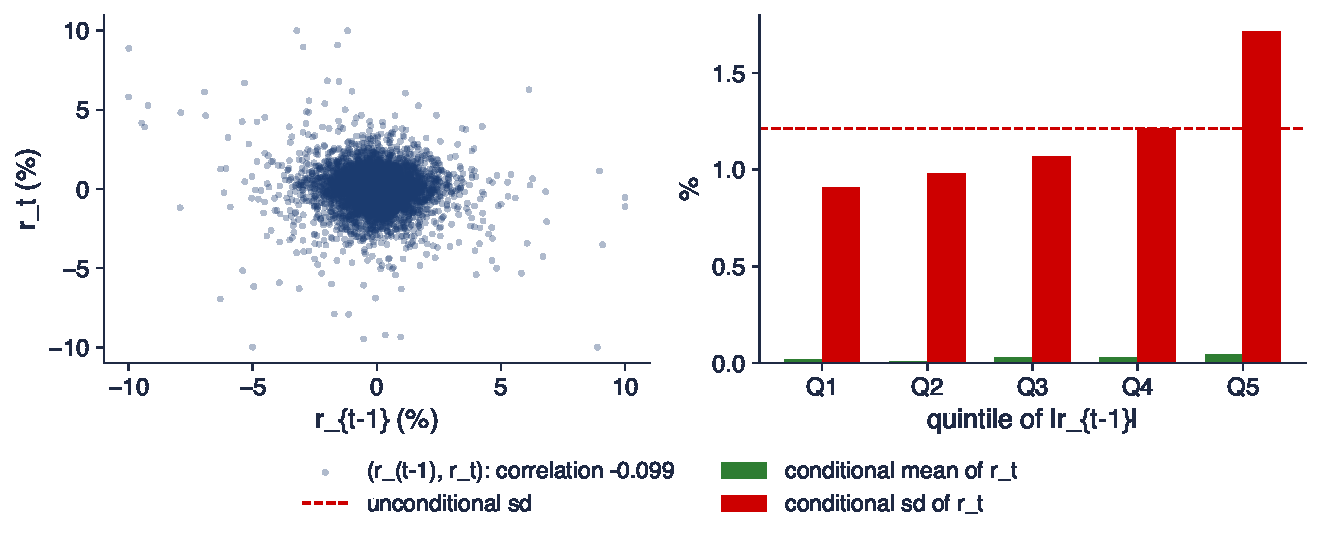
\includegraphics[width=1.0\textwidth,height=0.52\textheight,keepaspectratio]{ch4_sem_b1.pdf}
\end{center}
\vspace{-2mm}

\end{column}
\begin{column}{0.50\textwidth}
\begin{itemize}
    \item $n = 6\,714$, banda $\pm 0{,}024$; $\text{Corr}(r_t, r_{t-1}) = -0{,}099$; $\text{Corr}(r_t^2, r_{t-1}^2) = 0{,}313$
    \item Mediile condiționate Q1--Q5: $0{,}021; 0{,}006; 0{,}029; 0{,}027; 0{,}042$ (\%)
    \item Abaterile standard condiționate: $0{,}91; 0{,}98; 1{,}07; 1{,}21; 1{,}71$; Q5/Q1 $= 1{,}88$
    \item Varianța totală $1{,}4691 = 1{,}4690$ (în interiorul grupurilor) $+ 0{,}00013$ (între grupuri, 0{,}01\%)
    \item Interpretare: varianța este previzibilă, media aproape deloc; corelația negativă la decalajul 1 vine din zilele de criză cu reveniri mari, deci randamentele nu sînt independente
\end{itemize}
\end{column}
\end{columns}\sfmquantlet{Ch_04}{SFM_ch4_seminar}
\end{frame}

\begin{frame}{B2: aceeași analiză pentru DAX, BET și Bitcoin [Propus]}
\itemsize{\footnotesize}
\begin{itemize}
\item \textbf{Întrebarea}: arată DAX, BET și Bitcoin același tipar ca S\&P 500?
\item \textbf{Date}: randamente logaritmice zilnice, 2000--2026 (Bitcoin din 2014); model: B1
\item \textbf{Cerințe}
\begin{enumerate}
    \item Calculați ambele corelații la decalajul 1 și banda pentru fiecare serie.
    \item Calculați abaterea standard condiționată în Q1 și Q5 și raportul lor.
    \item Calculați ponderea varianței explicate de mediile chintilelor.
    \item Interpretare: de ce este BET singura serie cu $\text{Corr}(r_t, r_{t-1})$ clar pozitivă?
\end{enumerate}
\item \textbf{Raportați}: un tabel și o frază
\item Notebook: secțiunea B2
\end{itemize}
\end{frame}

\ifsolutions
\begin{frame}{B2: rezolvare [Propus]}
\itemsize{\footnotesize}
\begin{center}
\footnotesize
\begin{tabular}{lrrrrrrr}
\toprule
Seria & $\rho(r)$ & $\rho(r^2)$ & banda & sd Q1 & sd Q5 & Q5/Q1 & între \% \\
\midrule
DAX & $-0{,}017$ & $0{,}149$ & $0{,}024$ & $1{,}12$ & $1{,}89$ & $1{,}69$ & $0{,}03$ \\
BET & $0{,}109$ & $0{,}331$ & $0{,}024$ & $0{,}93$ & $2{,}25$ & $2{,}43$ & $0{,}08$ \\
Bitcoin & $-0{,}022$ & $0{,}137$ & $0{,}030$ & $3{,}28$ & $4{,}36$ & $1{,}33$ & $0{,}10$ \\
\bottomrule
\end{tabular}
\end{center}
\begin{itemize}
    \item Toate cele trei serii: corelația pătratelor randamentelor depășește mult banda, varianța este mai mare după mișcări mari, iar mediile chintilelor nu explică aproape nimic
    \item BET: cea mai puternică dependență a volatilității (Q5/Q1 = 2{,}43)
    \item Interpretare: $\rho(r)$ pozitivă pentru BET reflectă lichiditatea redusă: prețurile acțiunilor nelichide reacționează cu întîrziere, deci indicele preia știrile de ieri
\end{itemize}\sfmquantlet{Ch_04}{SFM_ch4_seminar}
\end{frame}
\fi

\begin{frame}{B3: probabilitatea unei pierderi lunare prin Monte Carlo [Rezolvat]}
\itemsize{\footnotesize}
\begin{itemize}
\item \textbf{Întrebarea}: cît de probabilă este o pierdere de peste 10\% în 21 de zile pentru S\&P 500 și depinde răspunsul de model?
\item \textbf{Date}: randamentele logaritmice zilnice ale S\&P 500, 2000--2026; 100\,000 de luni simulate
\item \textbf{Cerințe}
\begin{enumerate}
    \item Calculați probabilitatea exactă în ipoteza unor randamente zilnice Normale i.i.d., cu media și abaterea standard de selecție.
    \item Estimați-o prin Monte Carlo în același model și raportați eroarea standard.
    \item Estimați-o prin reeșantionarea cu întoarcere a 21 de zile observate (transformarea inversă empirică).
    \item Calculați ponderea ferestrelor de 21 de zile suprapuse din date cu o pierdere de peste 10\%.
    \item Interpretare: care diferențe se datorează erorii de simulare și care erorii de model?
\end{enumerate}
\item \textbf{Raportați}: patru probabilități, două erori standard, o frază
\item Notebook: secțiunea B3
\end{itemize}
\end{frame}

\begin{frame}{B3: rezolvare [Rezolvat]}
\itemsize{\scriptsize}
\begin{center}
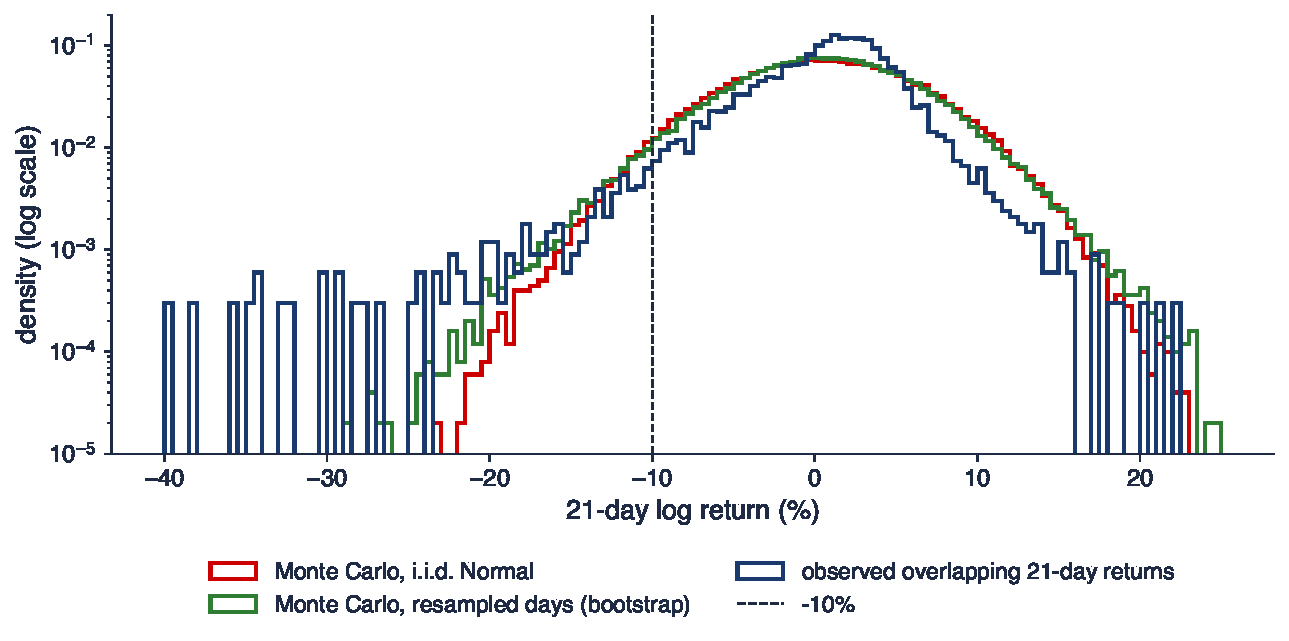
\includegraphics[width=0.96\textwidth,height=0.40\textheight,keepaspectratio]{ch4_sem_b3.pdf}
\end{center}
\vspace{-2mm}
\begin{itemize}
    \item Distribuția Normală, exact: 2{,}922\%; Monte Carlo cu distribuția Normală: 2{,}917\% (eroarea standard 0{,}053\%); bootstrap: 3{,}184\% (eroarea standard 0{,}056\%)
    \item În date: 2{,}67\% din cele 6\,694 de ferestre suprapuse (179 de ferestre, concentrate în cîteva episoade); luni care nu se suprapun: 3{,}45\% din 319
    \item Interpretare: Monte Carlo și valoarea exactă diferă cu mai puțin de o eroare standard (eroare de simulare); bootstrap-ul și modelul Normal diferă cu circa 3{,}5 erori standard (eroare de model: cozi zilnice mai groase); datele sînt zgomotoase pentru că ferestrele suprapuse sînt dependente
\end{itemize}\sfmquantlet{Ch_04}{SFM_ch4_seminar}
\end{frame}

\begin{frame}{B4: testați un generator de numere aleatoare [Propus]}
\itemsize{\footnotesize}
\begin{itemize}
\item \textbf{Întrebarea}: poate un generator să treacă testele simple și să fie totuși inutilizabil?
\item \textbf{Date}: RANDU, $x_{k+1} = 65539\,x_k \bmod 2^{31}$, sămînța 1, 100\,000 de numere; NumPy PCG64 cu aceeași sămînță; model: B3
\item \textbf{Cerințe}
\begin{enumerate}
    \item Calculați media, varianța și corelația la decalajul 1 pentru ambele șiruri și comparați-le cu $1/2$, $1/12$ și 0.
    \item Numărați valorile distincte ale lui $9u_k - 6u_{k+1} + u_{k+2}$ pentru ambele generatoare.
    \item Găsiți perioada generatoarelor LCG $(a, c, M) = (5, 1, 16)$, $(5, 0, 16)$ și $(4, 1, 16)$ pornite din 7.
    \item Interpretare: de ce nu detectează testele unidimensionale defectul RANDU?
\end{enumerate}
\item \textbf{Raportați}: un tabel cu șase statistici, două numărători, trei perioade, o frază
\item Notebook: secțiunea B4
\end{itemize}
\end{frame}

\ifsolutions
\begin{frame}{B4: rezolvare [Propus]}
\itemsize{\footnotesize}
\begin{center}
\footnotesize
\begin{tabular}{lrrrr}
\toprule
Generator & media & varianța & $\rho(1)$ & valori distincte \\
\midrule
RANDU & $0{,}5019$ & $0{,}0833$ & $0{,}0008$ & 15 \\
PCG64 & $0{,}5000$ & $0{,}0834$ & $0{,}0030$ & 99\,571 \\
\bottomrule
\end{tabular}
\end{center}
\begin{itemize}
    \item Ambele trec testele pentru momente și pentru corelația la decalajul 1 ($1/12 = 0{,}0833$); combinația RANDU ia doar 15 valori: tripletele lui stau pe 15 plane
    \item Perioade: (5, 1, 16): 16; (5, 0, 16): 4; (4, 1, 16): 1
    \item Interpretare: defectul este în distribuția comună a numerelor consecutive; testele distribuției marginale sau ale unui singur decalaj nu îl pot detecta; orice simulare tridimensională cu RANDU este deformată
\end{itemize}\sfmquantlet{Ch_04}{SFM_ch4_seminar}
\end{frame}
\fi

\begin{frame}{B5: este BET o mișcare browniană geometrică? [Rezolvat]}
\itemsize{\footnotesize}
\begin{itemize}
\item \textbf{Întrebarea}: ce trăsături ale BET poate reproduce un GBM cu aceeași tendință și volatilitate?
\item \textbf{Date}: închiderile BET, 2000--2026; 500 de traiectorii GBM de aceeași lungime
\item \textbf{Cerințe}
\begin{enumerate}
    \item Calibrați GBM: tendința logaritmică anuală și volatilitatea din randamentele logaritmice zilnice.
    \item Simulați 500 de traiectorii și calculați, pentru fiecare, excesul de aplatizare, $\text{Corr}(r_t^2, r_{t-1}^2)$ și drawdown-ul maxim.
    \item Plasați valorile reale în distribuțiile simulate (cuantilele de 5\% și 95\%).
    \item Interpretare: ce fapte stilizate ratează GBM și care indicator de risc este cel mai afectat?
\end{enumerate}
\item \textbf{Raportați}: doi parametri, trei comparații, o frază
\item Notebook: secțiunea B5
\end{itemize}
\end{frame}

\begin{frame}{B5: rezolvare [Rezolvat]}
\itemsize{\scriptsize}
\begin{center}
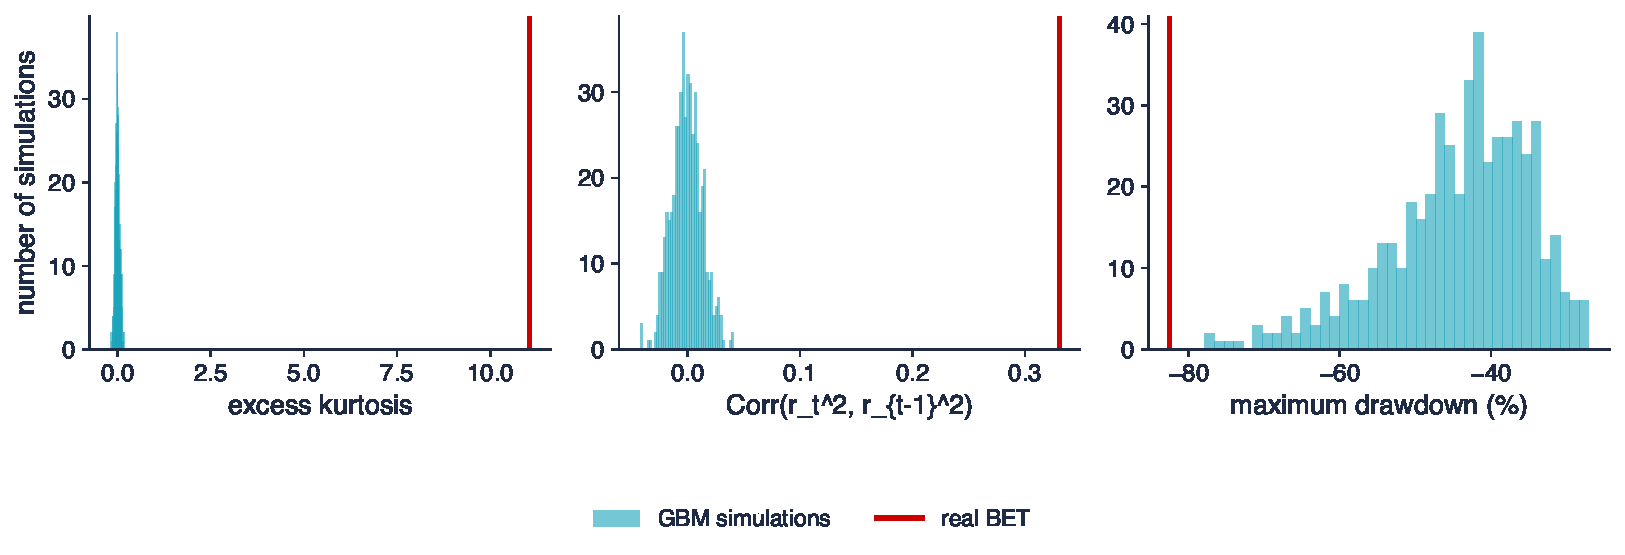
\includegraphics[width=0.96\textwidth,height=0.36\textheight,keepaspectratio]{ch4_sem_b5.pdf}
\end{center}
\vspace{-2mm}
\begin{itemize}
    \item $n = 6\,670$ zile; $\sigma = 22{,}1\%$, tendința logaritmică 16{,}0\% pe an
    \item Excesul de aplatizare: real $11{,}06$, intervalul GBM de 90\% $[-0{,}10; 0{,}10]$; $\text{Corr}(r_t^2, r_{t-1}^2)$: real $0{,}330$, GBM $[-0{,}022; 0{,}022]$
    \item Drawdown-ul maxim: real $-82{,}5\%$, mediana GBM $-42{,}7\%$, intervalul $[-62{,}8\%; -31{,}4\%]$
    \item Interpretare: GBM nu reproduce deloc cozile groase și volatility clustering; crahul din 2008 face drawdown-ul real mai adînc decît al oricărei traiectorii simulate, deci o limită de risc calculată cu GBM ar fi fost mult prea largă
\end{itemize}\sfmquantlet{Ch_04}{SFM_ch4_seminar}
\end{frame}

\begin{frame}{B6: crește varianța liniar cu orizontul? [Propus]}
\itemsize{\footnotesize}
\begin{itemize}
\item \textbf{Întrebarea}: este valabilă relația $\text{Var}(\text{randament pe } h \text{ zile}) = h\,\text{Var}(\text{randament zilnic})$, așa cum implică un mers aleator cu creșteri i.i.d.?
\item \textbf{Date}: randamentele logaritmice zilnice ale S\&P 500, BET, Bitcoin; blocuri disjuncte de $h = 5$, 21 și 63 de zile; model: B5
\item \textbf{Cerințe}
\begin{enumerate}
    \item Calculați raportul $\text{Var}(h \text{ zile})/(h\,\text{Var}(1 \text{ zi}))$ pentru fiecare serie și orizont.
    \item Folosiți eroarea standard aproximativă $\sqrt{2/(m - 1)}$ a unui raport de varianțe cu $m$ blocuri pentru a evalua cît de departe este raportul de 1.
    \item Interpretare: ce spune un raport peste 1 sau sub 1 despre autocorelația randamentelor?
\end{enumerate}
\item \textbf{Raportați}: un tabel $3 \times 3$ și două fraze
\item Notebook: secțiunea B6
\end{itemize}
\end{frame}

\ifsolutions
\begin{frame}{B6: rezolvare [Propus]}
\itemsize{\footnotesize}
\begin{center}
\footnotesize
\begin{tabular}{lrrr}
\toprule
Seria & $h = 5$ & $h = 21$ & $h = 63$ \\
\midrule
S\&P 500 & $0{,}84$ & $0{,}80$ & $0{,}66$ \\
BET & $1{,}15$ & $1{,}37$ & $1{,}68$ \\
Bitcoin & $0{,}96$ & $1{,}16$ & $1{,}28$ \\
eroarea standard aprox. (S\&P 500) & $0{,}04$ & $0{,}08$ & $0{,}14$ \\
\bottomrule
\end{tabular}
\end{center}
\begin{itemize}
    \item S\&P 500 sub 1 (revenire la medie pe cîteva săptămîni, mai ales din revenirile de după crize); BET peste 1 și în creștere (autocorelație pozitivă, lichiditate redusă); Bitcoin, la circa două erori standard de 1
    \item Interpretare: $\text{Var}(\sum r) = h\sigma^2 + 2\sum_{i<j}\text{Cov}(r_i, r_j)$; autocorelațiile pozitive împing raportul peste 1, cele negative sub 1
    \item Acesta este testul raportului varianțelor din \sfmchlink{https://danpele.github.io/SFM/RO/Cursuri/capitol7_piete_eficiente_mers_aleator_vr.pdf}{Capitolul 7}, unde se folosesc erorile standard exacte ale testului
\end{itemize}\sfmquantlet{Ch_04}{SFM_ch4_seminar}
\end{frame}
\fi


%=============================================================================
\section{Partea C: întrebări deschise și critica unui răspuns AI}
%=============================================================================

\begin{frame}{C1: cît de des apare un an nefavorabil? [Propus]}
\itemsize{\footnotesize}
\begin{itemize}
\item \textbf{Întrebarea}: dă GBM probabilitatea corectă a unui drawdown de peste 20\% (sau 40\%) în cursul unui an calendaristic?
\item \textbf{Date}: S\&P 500, DAX, BET, Bitcoin, ani calendaristici compleți 2000--2025 (Bitcoin 2015--2025); modele: B3, B5
\item \textbf{Cerințe}
\begin{enumerate}
    \item Calculați drawdown-ul maxim din fiecare an calendaristic și ponderea anilor cu peste 20\% și cu peste 40\%.
    \item Simulați 10\,000 de traiectorii de un an în GBM și în bootstrap-ul i.i.d. al randamentelor zilnice și calculați aceleași două probabilități.
    \item Comparați datele și modelele cu un test binomial.
    \item Propuneți un model care ar putea reproduce ambele probabilități.
    \item Interpretare: ce spune diferența dintre bootstrap și date despre volatility clustering?
\end{enumerate}
\item \textbf{Raportați}: un tabel, două valori $p$ binomiale, un scurt plan de proiect
\item Notebook: secțiunea C1
\end{itemize}
\end{frame}

\ifsolutions
\begin{frame}{C1: analiză de referință [Propus]}
\itemsize{\footnotesize}
\begin{center}
\footnotesize
\begin{tabular}{lrrrrrrr}
\toprule
Seria & ani & date 20\% & GBM & boot. & date 40\% & GBM & boot. \\
\midrule
S\&P 500 & 26 & 23{,}1 & 33{,}1 & 31{,}4 & 3{,}8 & 0{,}5 & 0{,}6 \\
DAX & 26 & 42{,}3 & 50{,}2 & 47{,}5 & 11{,}5 & 2{,}2 & 2{,}4 \\
BET & 26 & 46{,}2 & 33{,}5 & 31{,}8 & 3{,}8 & 0{,}7 & 0{,}8 \\
Bitcoin & 11 & 100{,}0 & 99{,}8 & 99{,}4 & 54{,}5 & 62{,}8 & 60{,}9 \\
\bottomrule
\end{tabular}
\end{center}
\begin{itemize}
    \item 20\%: GBM și bootstrap-ul dau rezultate apropiate; S\&P 500 a avut mai puțini ani nefavorabili decît prevăd ambele modele, BET mai mulți
    \item 40\%: ambele modele dau probabilități mult sub 3\% pentru indici, totuși 2008 (și, pentru DAX, 2001--2002) s-a produs: drawdown-urile adînci cer volatility clustering, nu doar cozi groase
    \item Direcții de proiect: simulări GARCH(1,1) și cu schimbare de regim, block bootstrap, mai mulți indici, un test formal pe 26 de ani
\end{itemize}\sfmquantlet{Ch_04}{SFM_ch4_seminar}
\end{frame}
\fi

\begin{frame}{C2: verificați un răspuns AI [Propus]}
\itemsize{\scriptsize}
\begin{itemize}
    \item Un student a cerut unui asistent AI să „rezume faptele de probabilitate despre S\&P 500 pentru un raport de risc”. Răspunsul:
    \item \aiprompt{(a) Corr(r\_t, r\_\{t-1\}) = -0{,}099, deci randamentele zilnice sînt independente și varianța de mîine nu poate fi prevăzută.}
    \item \aiprompt{(b) Prețul logaritmic este un mers aleator, deci varianța lui este aceeași la fiecare dată și procesul este staționar.}
    \item \aiprompt{(c) În GBM cu mu = 8\% și sigma = 19\%, valoarea mediană a unei investiții de 100 după 10 ani este 100 exp(0,8) = 222{,}6.}
    \item \aiprompt{(d) O probabilitate Monte Carlo de circa 3\% din 10.000 de traiectorii are o eroare standard de circa 0{,}0017.}
    \item \aiprompt{(e) Un portofoliu 50/50 din S\&P 500 și DAX are volatilitatea zilnică sqrt(0,25 x 1{,}22\textasciicircum 2 + 0,25 x 1{,}43\textasciicircum 2) = 0{,}94\%.}
    \item Cerințe
    \begin{itemize}
        \item 1. Pentru fiecare afirmație stabiliți dacă este corectă; dacă nu este, formulați afirmația corectă și dați valoarea corectă din notebook (secțiunea C2).
        \item 2. Raportați: o listă de cinci verdicte, fiecare cu un rînd de justificare.
    \end{itemize}
\end{itemize}
\end{frame}

\ifsolutions
\begin{frame}{C2: rezolvare [Propus]}
\itemsize{\footnotesize}
\begin{itemize}
    \item (a) Greșit: necorelat nu înseamnă independent; $\text{Corr}(r_t^2, r_{t-1}^2) = 0{,}31$, iar abaterea standard condiționată după zilele cele mai agitate este de 1{,}88 ori mai mare decît cea de după zilele cele mai calme
    \item (b) Greșit: $\text{Var}(S_t) = t\sigma^2$ crește cu $t$; un mers aleator nu este staționar (creșterile lui sînt)
    \item (c) Greșit: $100e^{\mu T} = 222{,}6$ este media; mediana este $100e^{(\mu - \sigma^2/2)T} = 185{,}8$
    \item (d) Corect: $\sqrt{0{,}03 \times 0{,}97/10\,000} = 0{,}0017$; eroarea scade ca $1/\sqrt{N}$, nu ca $1/N$
    \item (e) Greșit: lipsește termenul de covarianță; cu $\rho = 0{,}60$ volatilitatea este $1{,}19\%$, nu $0{,}94\%$: răspunsul AI subestimează riscul
\end{itemize}\sfmquantlet{Ch_04}{SFM_ch4_seminar}
\end{frame}
\fi


%=============================================================================
\section{Încheiere}
%=============================================================================

\begin{frame}{Idei de reținut}
\itemsize{\small}
\begin{itemize}
    \item Corelația zero nu înseamnă independență: verificați și pătratele sau valorile absolute
    \item Varianța condiționată a randamentelor reacționează la știrile de ieri; media condiționată aproape deloc
    \item Amestecurile de regimuri Normale dau cozi groase
    \item Monte Carlo: raportați eroarea standard; separați eroarea de simulare de eroarea de model
    \item GBM reproduce aproximativ traiectoria unui indice, dar nu și cozile, volatility clustering sau cele mai adînci drawdown-uri
    \item Un răspuns AI este o ciornă: verificați fiecare definiție, fiecare model și fiecare valoare numerică
\end{itemize}
\end{frame}

\begin{frame}{După seminar}
\itemsize{\small}
\begin{itemize}
    \item Cursul 4 dezvoltă fiecare temă de azi: distribuții, dependență, condiționare, Monte Carlo, arbori binomiali, mers aleator, procesul Wiener și GBM
    \item Încercați cerințele [Propus] în notebook; rezolvările se discută la seminar
    \item C1 poate deveni un proiect de echipă: simulări GARCH și cu schimbare de regim, block bootstrap, mai mulți indici
    \item Lectură: \refFHH, cap.~3--5; exerciții rezolvate: \refFHHex
\end{itemize}
\end{frame}


%=============================================================================
\section{Bibliografie}
%=============================================================================

\begin{frame}{Bibliografie}
\itemsize{\tiny}
\begin{itemize}
    \item Borak, S., Härdle, W.K., López-Cabrera, B. (2013). \href{https://doi.org/10.1007/978-3-642-33929-5}{\textit{Statistics of Financial Markets: Exercises and Solutions}}, 2nd ed. Springer.
    \item Cox, J.C., Ross, S.A., Rubinstein, M. (1979). \href{https://doi.org/10.1016/0304-405X(79)90015-1}{Option pricing: a simplified approach}. \textit{Journal of Financial Economics}, 7(3), 229--263.
    \item Franke, J., Härdle, W.K., Hafner, C.M. (2019). \href{https://doi.org/10.1007/978-3-030-13751-9}{\textit{Statistics of Financial Markets: An Introduction}}, 5th ed. Springer.
    \item Glasserman, P. (2003). \href{https://doi.org/10.1007/978-0-387-21617-1}{\textit{Monte Carlo Methods in Financial Engineering}}. Springer.
    \item Marsaglia, G. (1968). \href{https://doi.org/10.1073/pnas.61.1.25}{Random numbers fall mainly in the planes}. \textit{Proceedings of the National Academy of Sciences}, 61(1), 25--28.
\end{itemize}
\end{frame}

\end{document}
